%!TEX root = ../thesis.tex
%*******************************************************************************
%*********************************** Second Chapter *****************************
%*******************************************************************************
\chapter{Introduction to wind turbine modeling and design}
%*******************************************************************************
\hfill
\localtableofcontents
\newpage



%https://eolienne.f4jr.org/eolienne_etude_theorique

%https://www.geotechnique-journal.org/articles/geotech/pdf/2018/04/geotech190004s.pdf

%https://en.wikipedia.org/wiki/Wind-turbine_aerodynamics

%@book{hansen2015aerodynamics,
%  title={Aerodynamics of wind turbines},
%  author={Hansen, Martin OL},
%  year={2015},
%  publisher={Routledge}
%}

%============================================================%
%============================================================%
\section{Introduction}
%============================================================%
%============================================================%

Wind energy is a highly competitive industry with increasing regulations regarding its impact on ecosystems, land-use conflicts, landscapes, or air traffic management \citep{eolien_en_mer_2022}. 
During the long process to win calls for tenders, obtain construction permits, or throughout the wind farm exploitation, an advanced technical understanding of such systems might offer a competitive advantage. 

The operation of offshore wind turbines are driven by multiple physics coupled. 
This behavior results from different external solicitations which are highly turbulent and uncertain. 
Among them, the \textit{metocean} (abbreviation of meteorology and oceanography) environmental conditions play an important role. 
Note that many other types of solicitations also affect the exploitation of offshore wind turbines (e.g., corrosion of the structure, global scour, marine growth, stress concentration factor induced by the manufacturing quality, etc.). 

In this context, numerical models have been developed to certify the structural integrity of OWTs with respect to their solicitations. 
A wind farm project planned at given location should pass different validation procedures established by international standards such as the International Electrotechnical Commission \citep{iec_2019}. 
As wind turbine structures face a large amount of stress cycles in their lifetime (up to $10^8$ for 25 years of operation), this chapter will particularly focus on fatigue damage assessment.

\elias{The present thesis studied uncertainty quantification on two wind farm projects. 
First the Teesside wind farm, operating since xx in the North sea, second the theoretical wind farm of south Brittany , currently at the stage of calls for tenders.}

This chapter briefly introduces wind turbine modeling and design, in the following layout: 
Section \ref{sec:metocean_simulation} presents the methods used for wind and wave generation and wake simulation at a farm scale; 
Section \ref{sec:owt_modeling} recalls elements of theory associated with wind turbine modeling; 
Section \ref{sec:owt_design} introduces recommended practices regarding design and operation;
finally, Section \ref{sec:owt_uncertainties} gives a description of the various sources of uncertainties considered in this thesis. 
Considering the standard uncertainty quantification diagram presented in \fig{fig:UQ_methodo}, the material of this chapter is related to the step A (problem specification) and the step B (uncertainty quantification). 
%To go further this general introduction, the reader might refer to the following sources on the different topics 



%============================================================%
%============================================================%
\section{Metocean conditions simulation} \label{sec:metocean_simulation}
%============================================================%
%============================================================%

In the atmosphere, the wind is the air movements caused by the heterogeneous solar heating of Earth's surface. 
Winds usually move from high-pressure to low-pressure regions. 
Earth's rotation also impacts large-scale climate patterns, including winds, according to the well-known Coriolis effect. 
The wind is a highly variable resource, making its exploitation for energy production uncertain. 
This variability is both expressed in space and time with different behaviors depending on the scales studied. 

Regarding large timescales, yearly seasonal fluctuations of wind conditions are well-defined using probability distributions (typically Weibull distributions). 
Predictions at a shorter timescale are usually unreliable beyond a few days ahead. 
Under a few days, the spectral wind energy distribution per time unit is repesented by its power spectral density (PSD). 
Historically, the spectral study of horizontal wind by \citet{van_1957_wind_psd} for timescales between a few seconds and ten days revealed distinct ranges of behaviors. 
The PSD, such as the one illustrated in \fig{fig:wind_psd}, presents three main separated peaks, explaining how the wind energy is split. 
The two first peaks are named ``synoptic'' and ``diurnal'' peak, which respectively correspond to return periods around four days and one day.
While these two peaks are relatively close together, the third peak is completely separated. 
This peak describes the energy related to the wind turbulence, which evolves in the range below ten minutes. 
Considering this energy distribution, wind behaviors are often referred to as ``short-term'' (for turbulent wind) and ``long-term'' (otherwise). 
In wind turbine simulation, ten minutes simulations became a common practice to fully consider turbulent winds. 

Note that the spectrum presented in the research paper of \citet{van_1957_wind_psd} was build from wind measures near New York, USA. 
The same pattern between the three peaks is rather constant between sites, however, the geography (including the surface roughness, the topology, the proximity to the coast, etc.) may affect this distribution. 
At a larger timescale than one year, assessing trends becomes complicated. 
Wind resource assessment over decades are made more uncertain by the human-caused climate change \cite{nagababu_2023_climate_change}, which disrupts large weather trends and the occurrence of extreme events. 

\begin{figure}
    \centering
    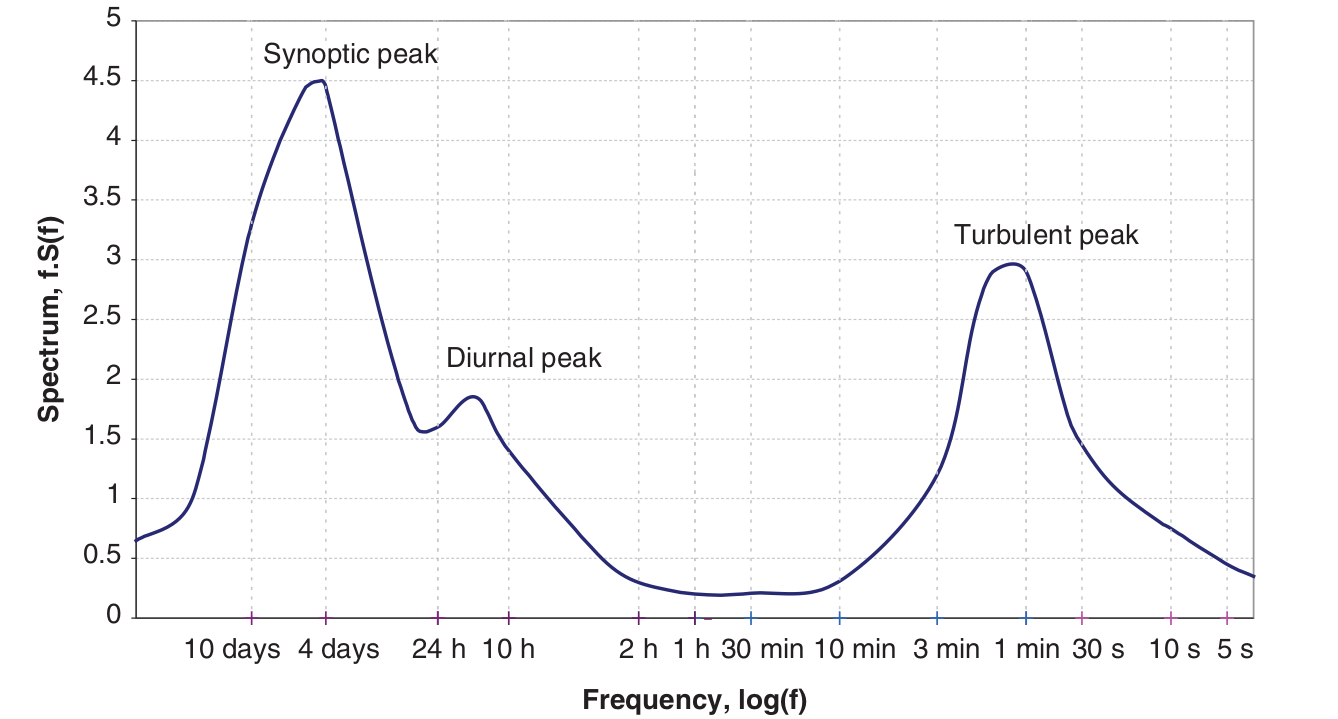
\includegraphics[width=0.7\textwidth]{./part1/figures/wind_spectrum.png}
    \caption{Wind spectrum from Brookhaven, USA (source: \citet{burton_2021_wind_handbook})}
    \label{fig:wind_psd}
\end{figure}

%\elias{Add something general regrading wave modeling?}



%============================================================%
\subsection{Turbulent wind generation}
%============================================================%

The wind turbulence is a complex and aleatory process, often described as chaotic, since a small perturbation of its initial conditions might have an important impact on the response. 
However, the wind over short-term periods (i.e., ten minutes periods) is usually assumed to be a Gaussian process with constant mean $\overline{U}$ and standard deviation $\sigma_U$ \citep{burton_2021_wind_handbook}. 
Its mean is modeled by the long-term wind conditions (i.e., mean wind speed), often described by a probabilistic model such as a Weibull distribution. 
Note that this assumption is based on the bimodal wind energy distribution observed in \fig{fig:wind_psd}, which might vary at some specific locations. 

The \textit{turbulence intensity} is a commonly used normalized statistic of the wind variability: 
\begin{equation}
    I = \frac{\sigma_U}{\overline{U}}.
\end{equation}

\begin{figure}
    \centering
    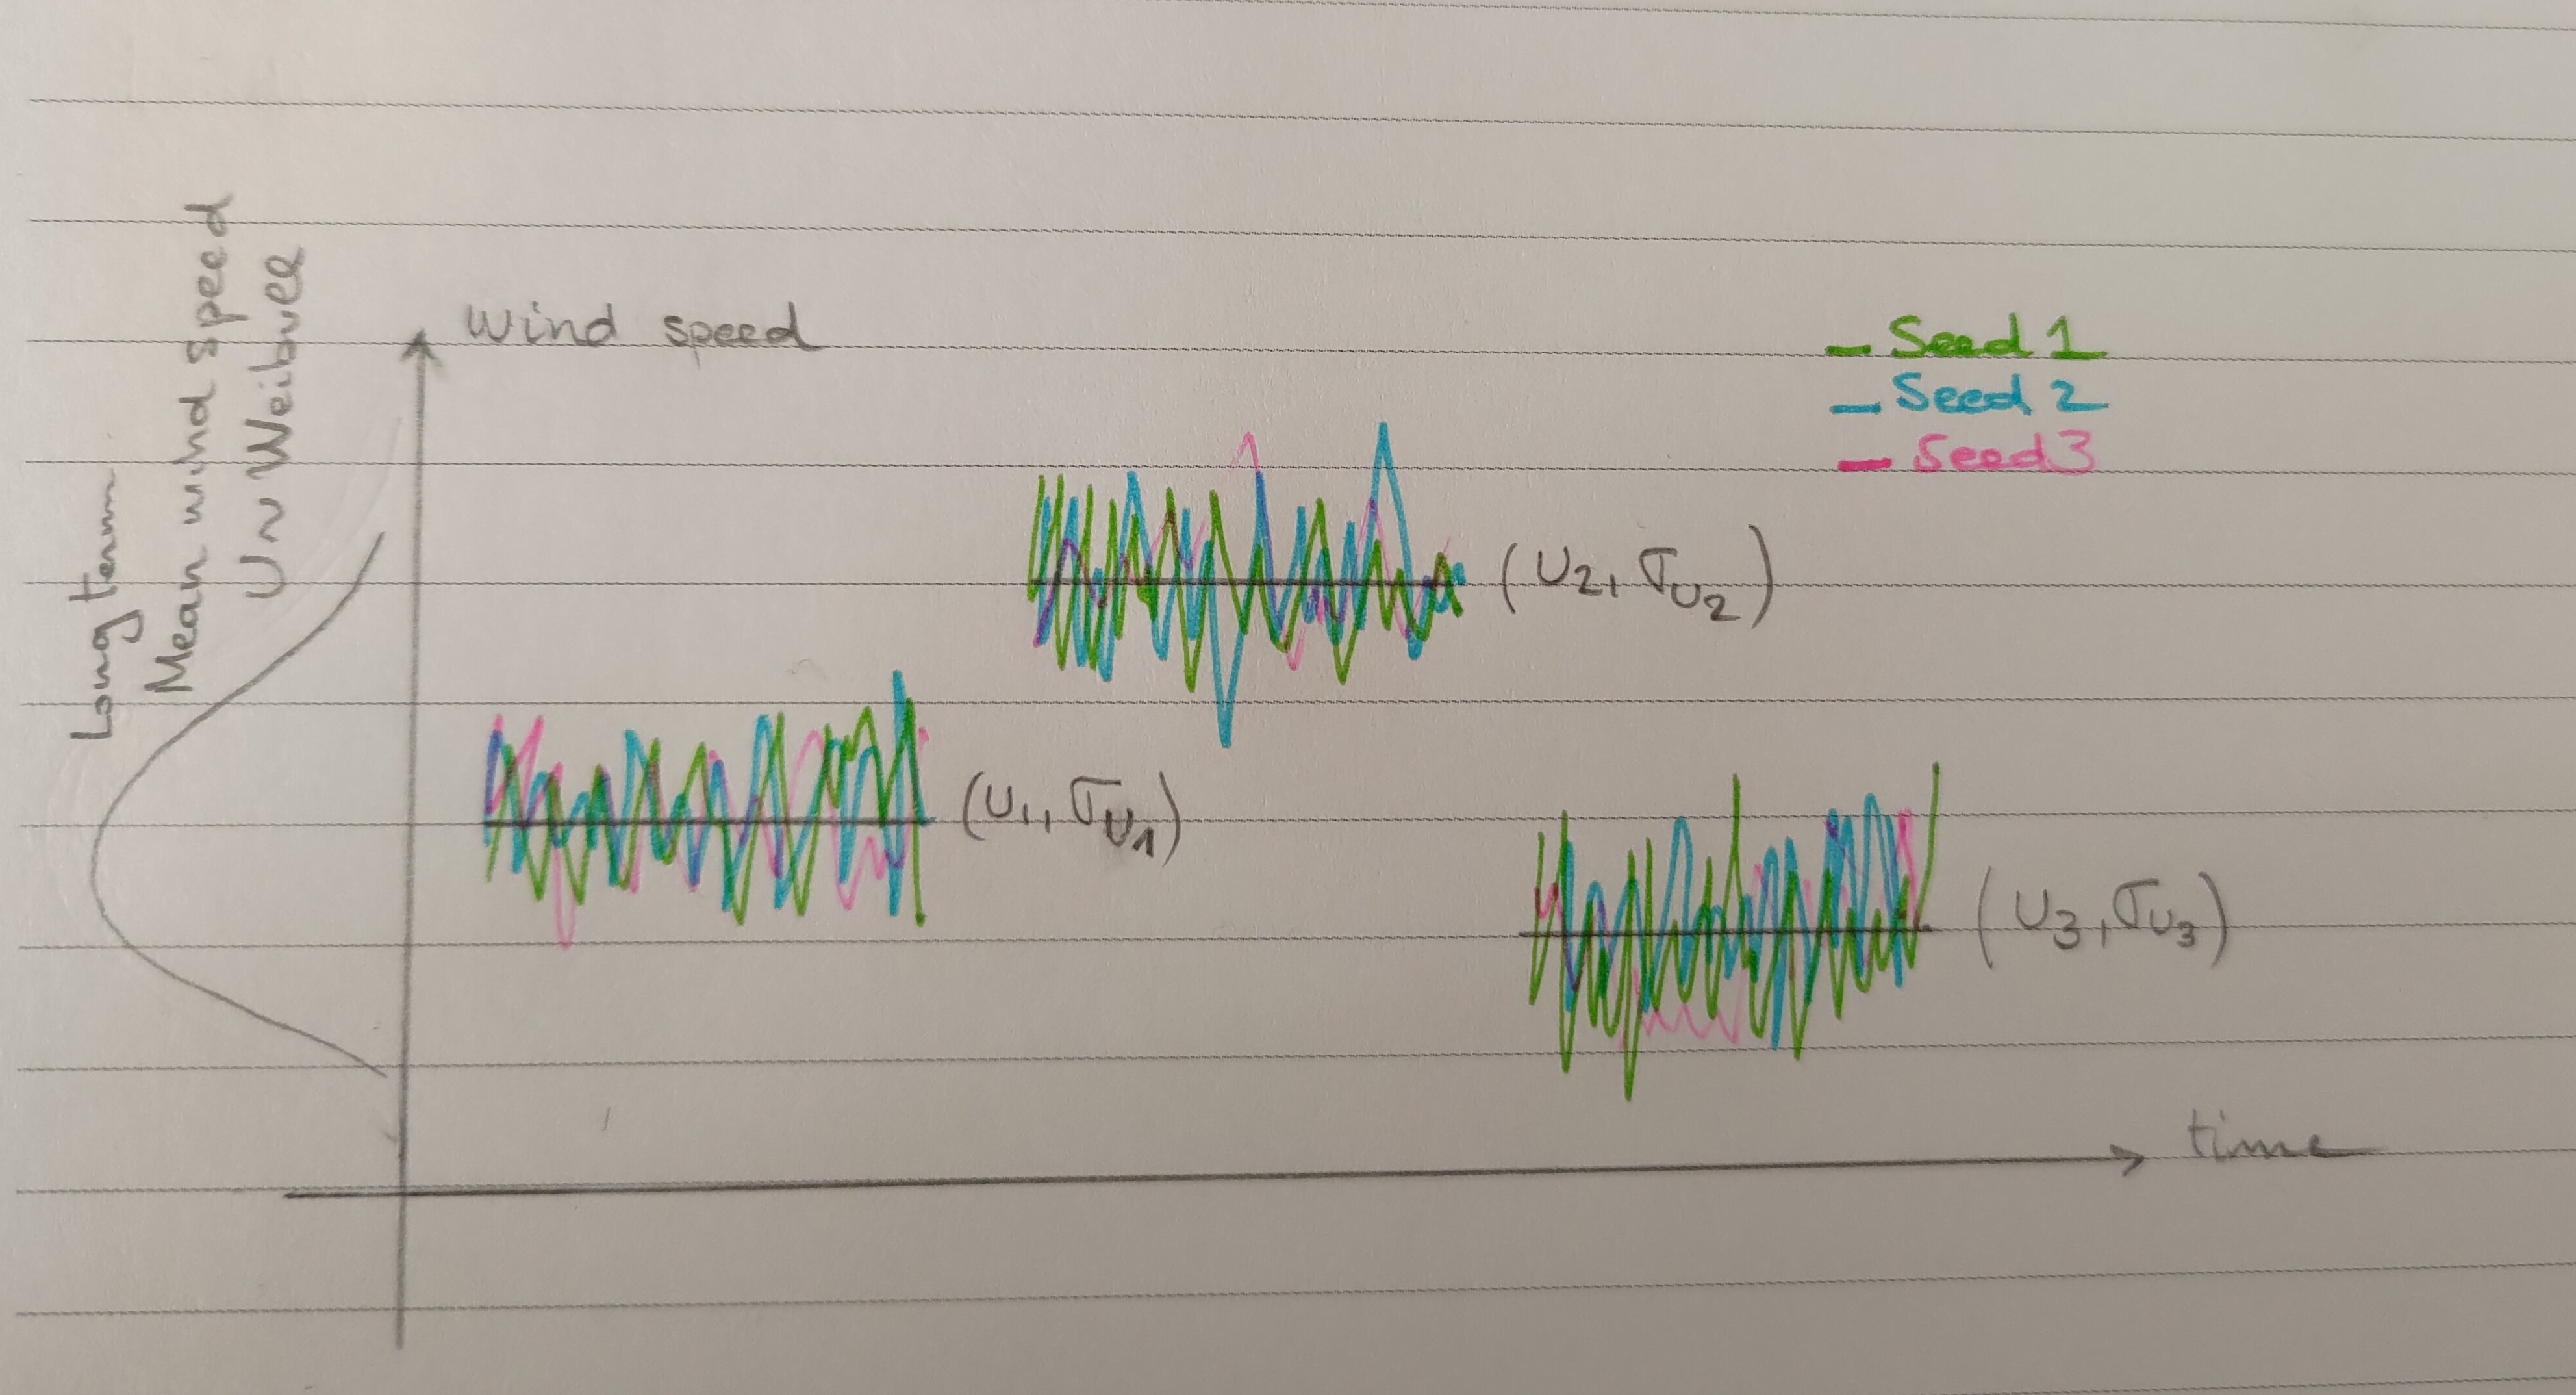
\includegraphics[width=0.7\textwidth]{./part1/figures/wind_long_short_term.jpg}
    \label{fig:wind_long_short_term}
    \caption{\elias{Representation to be confirmed and mentioned in the text}}
\end{figure}

As the wind depends on differences between pressure, humidity, air density, different models exist to represent vertical wind profiles. 
The vertical change in wind conditions is referred to as \textit{vertical wind shear}.
Assuming a constant standard deviation over the altitude, the power law is a widely used approximated shear model \citep{iec_2019}:
\begin{equation}
    \overline{U}(z) = \overline{U}_0 \left(\frac{z}{z_{\mathrm{0}}}\right)^\alpha,
\end{equation}
with $\overline{U}_0$ a well-defined mean wind speed at the height $z_{\mathrm{0}}$ (typically corresponding to a measurement height), 
$z$ the studied height (e.g., the turbine's hub-height), and $\alpha$ the vertical shear coefficient (defined according to measures or standards recommendations). 

To generate a turbulent wind field on a mesh around the turbine, the general mechanism is to apply inverse Fourier transforms on a turbulent wind spectrum.  
Two types of parametric spectrums are commonly used in wind energy: the \textit{Kaimal model} \citep{kaimal_1972} and the \textit{Mann model} \citep{mann_1998}. 
In this thesis, the Kaimal spectrum as defined in \cite{iec_2019} is used for turbulent wind generation over the Cartesian component $k \in \{u, v, w\}$:
\begin{equation}
    S_k(f) = \frac{4 \sigma_k^2 \frac{L_k}{\overline{U}}}{\left(1 + 6 f \frac{L_k}{\overline{U}}\right)^{5/3}},
    \label{eq:kaimal}
\end{equation} 
such that $f$ is the frequency, $\overline{U}$ is the longitudinal mean speed at hub-height, $L_k$ are the Kaimal length scales, and $\sigma_k$ standard deviations (see the complete definition in Annex C of \cite{iec_2019}). 
Along with the Kaimal wind speed spectrum, a spacial coherence model is usually defined in the frequency domain. 
Each couples of nodes in the mesh are correlated, for example, using an exponential coherence model (for further detail in Annex C from \cite{iec_2019}).

In this thesis, the full-field turbulent wind fields (i.e., over a regular mesh) are generated using TurbSim, a software developed by the National Renewable Energy Laboratory (NREL) \citep{turbsim_2009}. 
TurbSim generates time realizations by adapting the spectral method proposed in \citet{veers_1988_sandia} (relying on the inverse Fourier transforms of each component).   
Considering a wind spectrum (e.g., Kaimal model) and a vertical shear model (e.g., power law), TurbSim takes as inputs a mean wind speed, a turbulence standard deviation and a mean wind orientation. 
\fig{fig:turbsim_simu} illustrates the corresponding wind field generated by a ten-minutes TurbSim simulation, considering a set of input long-term conditions. 

\begin{figure}
    \centering
    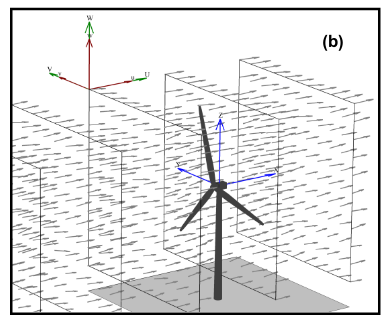
\includegraphics[width=0.5\textwidth]{./part1/figures/turbsim.png}
    \caption{Example of a turbulent wind field generated by TurbSim (source: \citet{turbsim_2009})}
    \label{fig:turbsim_simu}
\end{figure}

In their recent review of the challenges in wind energy, \citep{veers_2019_review} list some limits of the two spectral turbulence models recommended by the standards. 
First, their parameters were fitted using a restricted amount of data \citep{dimitrov_2017_turbulence_models_on_loads}. 
Second, the spacial coherence models associated with Kaimal models showed differences with turbulence measured on site \citep{saranyasoontorn_2004}.  
Finally, recent studies showed that the choice of spectral model impacts the resulting wind turbines loads \citep{doubrawa_2019}. 
These approximations generally tend to overestimate wind flows, leading to conservative designs.

To ensure the most realistic turbulent wind field generation, two research perspectives are actively explored. 
Authors recently developed hybrid methods, including measurement data to enhance spectral models \citep{dimitrov_2017_constrained_turbulence}. 
Alternatively, higher fidelity models were studied in this domain, see for example the use of vortex methods \citep{branlard_2017_book} and large eddy simulations (LES) \citep{doubrawa_2019,bui_2022_mesoscale_LES}.  
Such complex models allow the simulation of mesoscale conditions (e.g., at the farm scale), and extreme transient events (e.g., gusts and storms). 
However, their computational cost is often prohibitive in uncertainty quantification studies. 
When studying the wind resources at a wind farm scale, modeling wind energy losses induced by the turbines' wake becomes essential.


%============================================================%
\subsection{Wake modeling}
%============================================================%

The wake is caused by the extraction of the wind kinetic energy, reducing the wind speed and increasing the turbulence downstream of the turbines (see the illustration in \fig{fig:wake_illustration}). 
In a wind farm, this effect depends on the spacing between turbines, as well as the ambient wind speed and turbulence intensity. 
The turbines positioned at the center of the farm are the most impacted by the wake. 
As a wind farm owner, the consequence of the wake is twofold: a loss of energy production (in the range of 10 to 20 percents depending on the farm), and an increase of fatigue loads (due to the asymmetric loading from the created turbulences).

\begin{figure}%[h!]
    \centering
    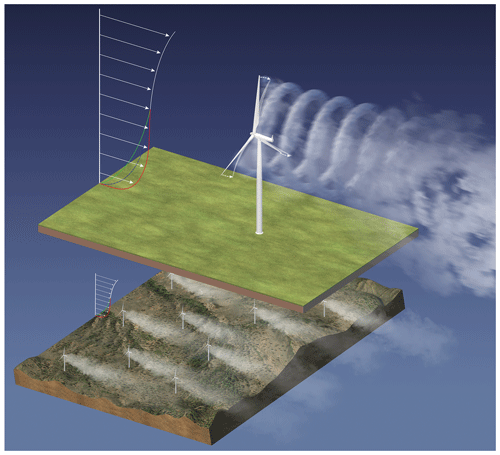
\includegraphics[width=0.5\textwidth]{./part1/figures/wake.png}
    \caption{Illustration of the wake created downstream a wind farm (source: \citet{veers_2019_review})} 
    \label{fig:wake_illustration}
\end{figure}

The initiation of the wake is a complex physical mechanism, however, the wake almost becomes axisymmetric after two turbine diameters downstream. 
At this stage, the wind speed deficit often presents a Gaussian profile centered on the hub \citep{burton_2021_wind_handbook}. 
Numerical models of different fidelities aim at simulating the wake. 
For example, computational fluid dynamics (CFD) models give a detailed description of the wake (including near the turbine) but require high computational efforts. 
In practice, simple analytical models (often called ``engineering models'') are widely used and recommended by standards (see e.g., Annex E in \citet{iec_2019}). 
These models mostly rely the equivalence between the thrust load on the turbine wind energy deficit. 
Since the seminal engineering model proposed by \citet{jensen_1983_wake}, multiple enhancements were proposed. 
A wide benchmark of the wake modeling solutions for different fidelities was performed in \citet{doubrawa_2020_benchmark} and \citet{hiperwind_2023_wp3}. 
The optimal tuning of these engineering models was studied using measurements from a Doppler wind lidar in \citet{zhan_2020_optimal_wake}. 
Different software programs propose wake engineering models, such as: FLORIS (developed by the NREL \citet{fleming_2020_FLORIS}), FarmShadow (developed by IFPEN). 

To take into account the wake effect, control strategies increasingly move from the turbine scale to the farm scale. 
This concept, called ``active wake control'', introduces small yaw misalignments (making the control of turbines individually suboptimal) to optimize the global wake inside the farm \citep{rott_2018_active_control,simley_2020_active_control,meyers_2022_active_control}. 


%============================================================%
\subsection{Irregular wave generation}
%============================================================%

The propagation of wind generated waves has long been studied in hydrodynamics, leading to various wave theories including Airy's, and Stokes'. 
Airy wave theory (also referred to as linear wave theory), models sea states under the hypothesis of small waves relatively to the water depth.  
This spectral approach superposes many regular waves, following the same wave spectrum, to model irregular waves. 
Standard statistics are used in oceanography to represent sea states and their corresponding wave spectra: 
the wave period $T_p$ (with respective frequency $f_p$), and the significant wave height $H_s$ (average over the highest third of the waves measured). 

The most commonly used parametric wave spectrum is called JONSWAP, after the Joint North Sea Wave Project \citep{jonswap_1973}: 
\begin{equation}
    S(f) = \delta \frac{H_s^2}{f} \left(\frac{f_p}{f}\right)^4 \exp\left[-\frac54 \left(\frac{f_p}{f}\right)^4 \right] \gamma^\alpha.
    \label{eq:jonswap}
\end{equation}
The JONSWAP spectrum is a correction of the Pierson-Moskowitz spectrum, adding the peak enhancement factor $\gamma^\alpha$. 
Further details regarding the numerical values to choose in \eq{eq:jonswap} are given in \citet{burton_2021_wind_handbook}. 
An illustration of the two spectra is presented in \fig{fig:jonswap}, revealing the artificial enhancement factor proposed in the JONSWAP model to better fit sea states measurements. 

\begin{figure}%[h!]
    \centering
    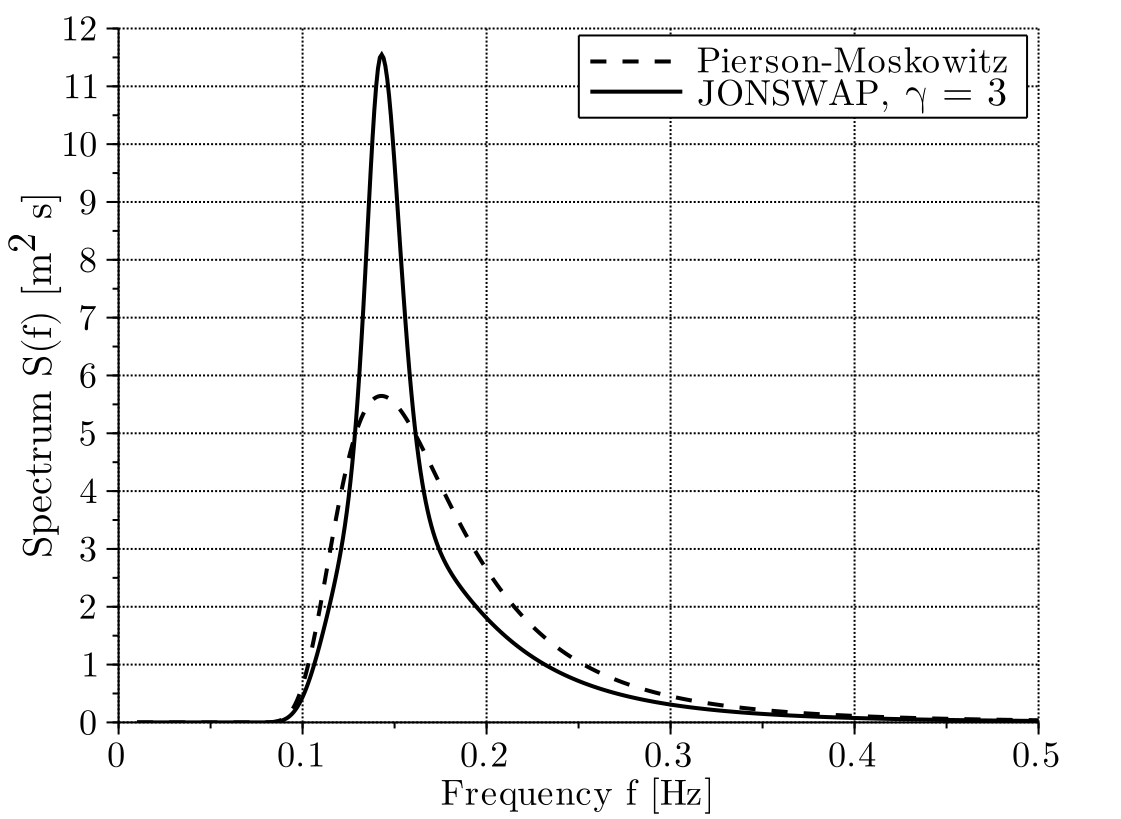
\includegraphics[width=0.45\textwidth]{./part1/figures/jonswap.png}
    \caption{Peirson-Moskowitz and JONSWAP spectra at significant wave height $H_s = 3$
    m and peak period $T_p = 7$ s (source: \citet{milano_thesis_2021})}
    \label{fig:jonswap}
\end{figure}

To take into account sea swell, meaning the waves resulting from weather conditions occurring far away, the unimodal wave spectra introduced in \eq{eq:jonswap} was improved. 
Swell waves usually present long wavelength, allowing them to propagate over long distances with little dissipation. 
Different methods allow to build a parametric bimodal distribution, with a mode in the low frequencies corresponding to the swell. 
\citet{guedes_2005_bimodal_jonswap} reviews different bimodal wave spectra, and compares their adequacy with measured sea states. 



%============================================================%
%============================================================%
\section{Wind turbine multi-physics modeling} \label{sec:owt_modeling}
%============================================================%
%============================================================%

Offshore wind turbine models are coupling multiple physics such as aerodynamics, hydrodynamics, mechanical elasticity, control and mooring dynamics for floating OWT. 
Similarly to the usual practices from the offshore oil \& gas industry, OWT have been first modeled in the frequency domain. 
At an early design stage, a study in the frequency domain gives a rough idea of the system's feasibility by computing its natural frequencies. 
An OWT should not have its natural frequencies in the same range as the main frequencies of the wave energy spectra. 
Otherwise, such systems can be subject to critical dynamic resonance, leading to their failure.

Beyond this preliminary check, frequency-domain approaches present limits for OWT modeling. 
As they rely on linear assumptions, they are unable to model the non-linearities and transient loading phases \citep{matha_2011_ISOPE}. 
These aspects happen to be essential in the design of OWT \citep{jonkman_2011_ISOPE}. 
As an alternative, the behavior of OWT systems are also simulated in the time domain. 

In the time domain, such systems may be models at different fidelities. 
The diagram in \fig{fig:owt_modeling_fidelities}, illustrates the increasing complexities for two physics involved in OWT modeling (aerodynamics and structural dynamics). 
To perform an uncertainty quantification around a wind turbine model, its fidelity is preferably low. 
At the wind turbine scale, the numerical model studied in this work is actually a chain of three models executed sequentially as illustrated in the diagram in \fig{fig:owt_chained_model}. 
\begin{itemize}
    \item \elias{TurbSim}
    \item \elias{DIEGO}
    \item \elias{Fatigue assessment}
\end{itemize}
Note that the wake should also be considered at the wind farm scale, as described earlier. 

\begin{figure}
    \centering
    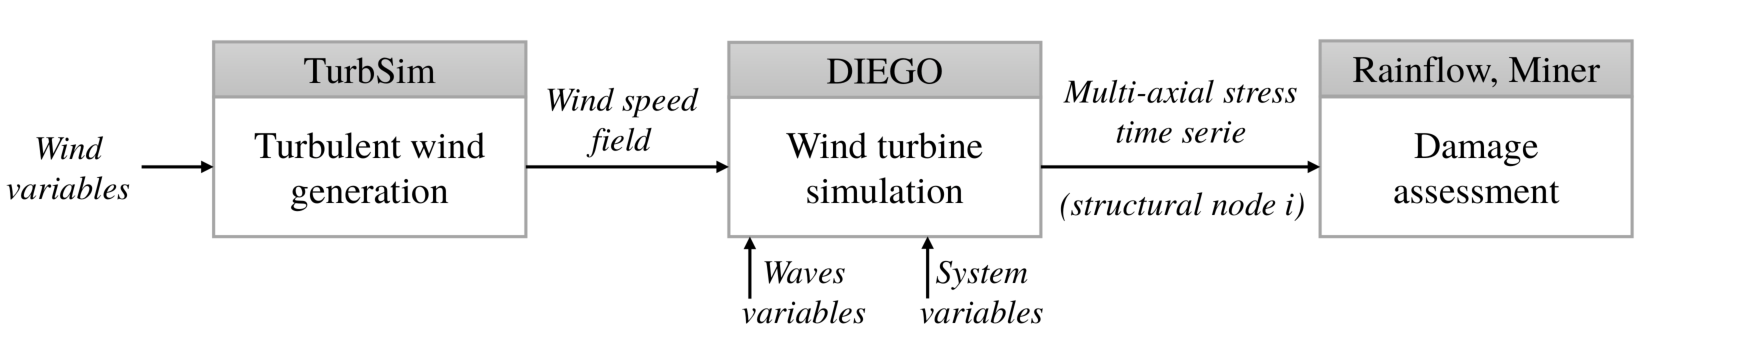
\includegraphics[width=0.8\textwidth]{./part1/figures/chained_model.pdf}
    \caption{Chained numerical model of offshore wind turbine.}
    \label{fig:owt_chained_model}
\end{figure}


\begin{figure}
    \centering
    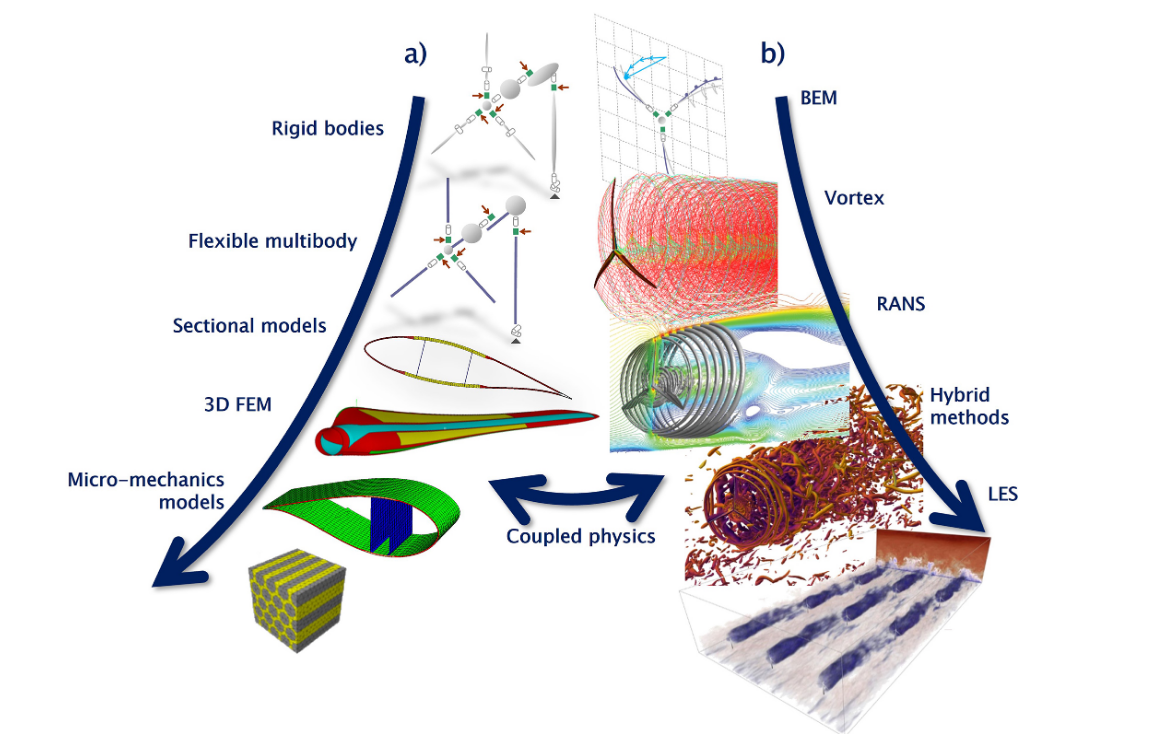
\includegraphics[width=0.7\textwidth]{./part1/figures/OWT_modeling_fidelities.png}
    \caption{Hierarchy of structural (a) and aerodynamic (b) wind energy systems models (source: \citet{veers_2019_review})}
    \label{fig:owt_modeling_fidelities}
\end{figure}



%============================================================%
\subsection{Aerodynamics of horizontal axis wind turbines}
%============================================================%

The blade element momentum theory mixes different concepts to compute the aerodynamic forces on the rotating blades of the wind turbine.
In this coupled physics models, the aerodynamics affects the structural response and vise-versa. 
To solve this problem, algorithms used in DIEGO first assess displacement of elementary blades, to recover the lift and drag coefficients. 
The elementary loads are then integrated over each blade and communicated to the structure's finite element model (FEM).


\paragraph{Momentum theory.}
%------------------------------------------------------------%
At the core of wind turbine's aerodynamics, the concept of \textit{momentum theory}, also called \textit{actuator disk theory} assumes that the air stream passing thought the rotor disk is bounded by a stream tube of circular surface (not mixing with the ambient air). 
\fig{fig:actuator_disk} is a longitudinal representation of the actuator disk and the way it affects the air stream upstream and downstream the rotor. 
The associated momentum theory assumes the conservation of airflow at any cross-section (of area $A$) during a time period. 
Through the actuator disk, the wind speed slows down and a drop in static pressure is created, at the origin of the wake. 
This pressure drop generates an axial force (called \textit{axial thrust force}) and a torque on the actuator disk.

\begin{figure}[!h]
    \centering
    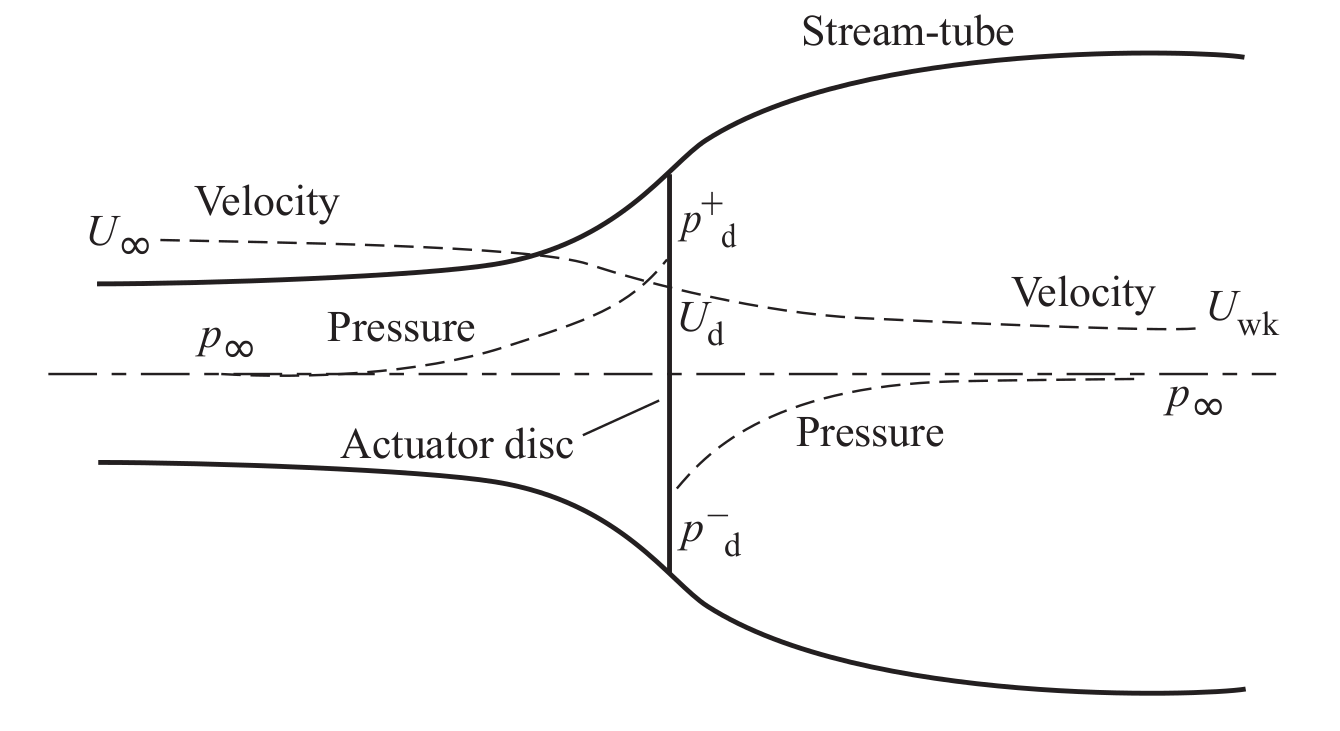
\includegraphics[width=0.6\textwidth]{./part1/figures/actuator_disk.png}
    \caption{Actuator disk model of the energy extraction (source: \citet{burton_2021_wind_handbook}). Longitudinal evolution of the air pressure and wind speed along the wind stream.}
    \label{fig:actuator_disk}
\end{figure}
Considering the upstream flow, the flow at the rotor disk and the airflow in the wake, respectively denoted by the subscripts $\{\infty, d, \mathrm{wake}\}$, the following equality comes:  
\begin{equation}
    \rho A_\infty U_\infty = \rho A_d U_d = \rho A_{\mathrm{wake}} U_{\mathrm{wake}},
\end{equation}
where $U$ is the wind speed, $A$ the stream-tube area, and $\rho$ the air density. 
The wind speed in at the rotor disk can be expressed using the induction factor $a$ in the following expression: 
\begin{equation}
    U_d = U_\infty (1 - a), \, 0\leq a \leq 1.
\end{equation}
Using the momentum theory and Bernoulli's incompressible flow equation, one can express the aerodynamic thrust $T$ and power $P$ (see \citet{milano_thesis_2021}): 
\begin{subequations}
    \begin{align}
        T&=(p_d^+ - p_d^-) A_d = 2 \rho A_d U_\infty^2 a (1- a)\\
        P&= T U_d = 2 \rho A_d U_\infty^3 a (1- a)^2
    \end{align}
    \label{eq:momentum_theory}
\end{subequations}
The widely used power coefficient (respectively thrust coefficient) is the ratio of the power captured by the turbine against to the total kinetic wind power available in the stream tube: 
\begin{subequations}
    \begin{align}
        C_P &= \frac{P}{\frac12 \rho A_d U_\infty^3} = 4a (1-a)^2,\\
        C_T &= \frac{T}{\frac12 \rho A_d U_\infty^2} = 4a (1-a). 
    \end{align}
\end{subequations} 
Betz's law is a theoretical limit value of the power coefficient, obtained by cancelling the power coefficient gradient. 
To this day, no wind turbine has exceeded this limit value: $C_P^{\mathrm{Betz}} = 0.593$ \citep{burton_2021_wind_handbook}.  



\paragraph{Blade element theory.}
%------------------------------------------------------------%
Assuming a purely two-dimensional flow (meaning that the forces are only determined by the lift and drag coefficients), the blade element theory expresses the thrust $\dd T$ and torque $\dd Q$ applied on a blade element.

Let us consider a wind turbine with $B$ blades, with pic length R and pitch angle $\beta$. 
Assuming the blade element represented in \fig{fig:blade_theory} at the blade length $r$, with airfoil chord $c$, angle of attack $\alpha$,  lift $C_L$ and drag $C_D$ coefficients, lift $L$ and drag $D$ forces, and the axial and tangential induction factors $a$ and $a'$. 
Under these assumptions, the axial thrust and torque exerted on a blade element are:
\begin{subequations}
    \begin{align}
        \dd T &= \frac12 \rho W^2 B\, c \left(C_L \cos(\varphi) + C_D \cos(\varphi)\right) \dd r,\\
        \dd Q &= \frac12 \rho W^2 B\, c \left(C_L \sin(\varphi) + C_D \sin(\varphi)\right) \dd r.
    \end{align}
    \label{eq:blade_element}    
\end{subequations}

\begin{figure}[h!]
    \begin{subfigure}[b]{0.5\textwidth}
        \centering
        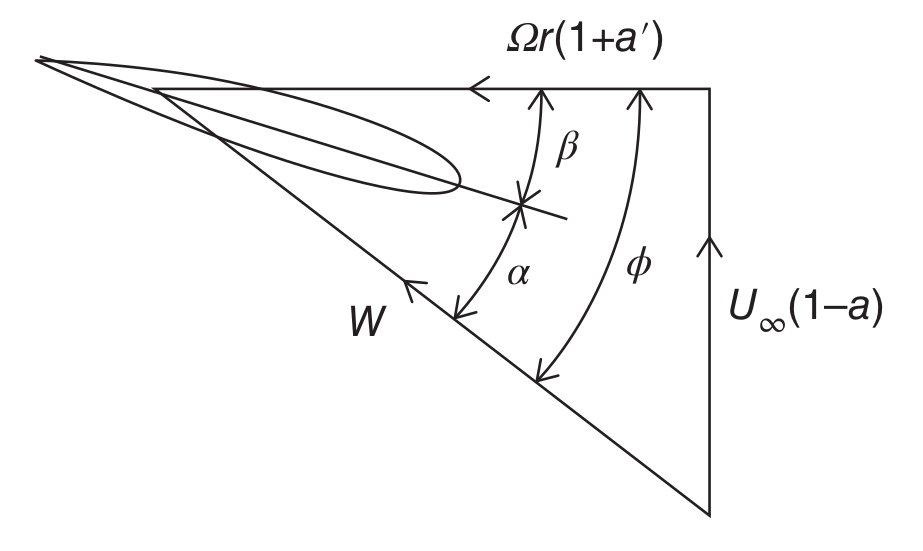
\includegraphics[width=0.9\linewidth]{./part1/figures/speed_triangle.png}
        \caption{Speed triangle}
    \end{subfigure}
    \begin{subfigure}[b]{0.5\textwidth}
        \centering
        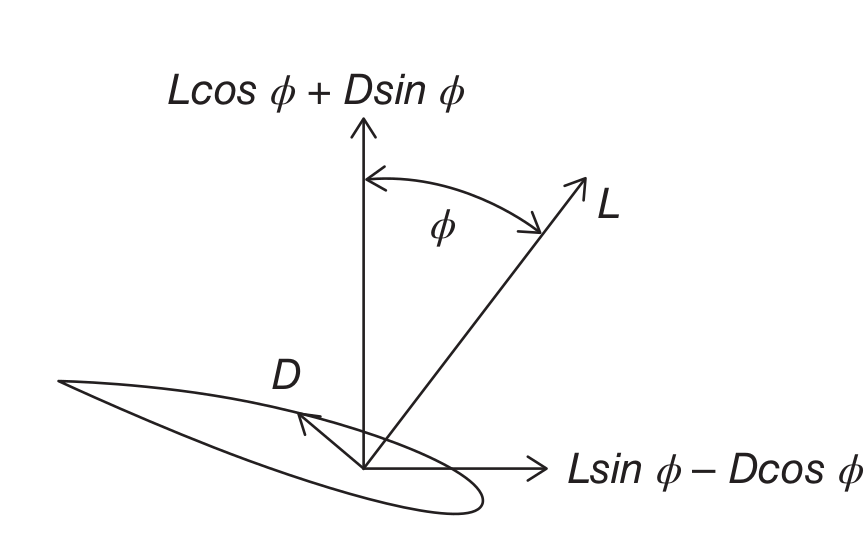
\includegraphics[width=0.9\linewidth]{./part1/figures/aerodyn_blade.png}
        \caption{Aerodynamic forces}
    \end{subfigure}
    \caption{Blade element forces. With the lift and drag forces $L$ and $D$, the flow angle $\phi$, the pitch angle $\beta$ and the angle of attack $\alpha$ (source: \citet{burton_2021_wind_handbook}).}
    \label{fig:blade_theory}
\end{figure}
\textit{Blade element momentum theory} (BEMT) combines the results from blade element theory in \eq{eq:blade_element} with the results from momentum theory in \eq{eq:momentum_theory} to obtain the induction factors $a$ and $a'$. 
The resolution of this sytem of equations is often solved by iterative approaches (e.g., \cite{dai_2011_BEMT}). 
Global axial thrust over the blade are then computed by integrating the elementary loads over all the elements. 
Note that various corrections are applied to the BEMT model, for example to take into account the non-homogeneous loss of momentum over the rotor disk. 
The BEMT also fails to model non-linear aerodynamic effects, occurring with sudden change of angle of attack. 
Such effects are sometimes called ``dynamic stall'' and are represented in DIEGO by the Beddoes-Leishman model (see \citet{burton_2021_wind_handbook} for further details).  

\elias{\paragraph{Aerodynamic damping?}}
%------------------------------------------------------------%
% See Petrovska p.51 


%============================================================%
\subsection{Hydrodynamics}
%============================================================%

Morison's equations is a widely-used semi-empirical model to assess the hydrodynamic forces on thin fixed structures such as offshore oil platforms and wind turbines. 
Considering a slender cylindrical structure of diameter $D$, a flow velocity $u(t)$, the drag and inertial coefficients $C_m$ and $C_D$, the axial force (parallel to the flow direction) is given by:   
\begin{equation}
    F\,=\,C_{m}\,\rho \,{\frac {\pi }{4}}D^{2}\,{\frac{\dd u}{\dd t}}\,+\,C_{d}\,{\frac 12}\,\rho \,D\,u\,|u|.
\end{equation}
Standard values for the drag and inertial coefficients are often considered \citep{dnv_2013_offshore_design}. 
DIEGO uses Morison’s equation together with first order potential solution to perform hydrodynamical simulations in the time domain.
An extended introduction to hydrodynamics of fixed slender structures, as well as large floating structures is given in the Chapter 1 from \citep{milano_thesis_2021}.  

%============================================================%
\subsection{Control}
%============================================================%

To maximize their energy production under turbulent wind conditions, wind turbines rely on their control systems. 
This aspect of wind turbines is usually kept confidential by manufacturers, as it gives them a competitive advantage.  
Nevertheless, the general control mode on a wind turbine depends on the wind speed. 
Two main ranges of operation are usually defined: first between the cut-in and rated wind speed, second between the rated and cut-off wind speed. 
Let us then recall the wind turbine power derived from the momentum theory: 
\begin{equation}
    P = \frac12 \rho A_d U_\infty^3 C_p(\lambda, \beta), 
    \label{eq:power_wt}
\end{equation}
with the power coefficient $C_p$, function of the pitch angle $\beta$ and the blade tip speed ratio $\lambda$, defined between the tangential speed on top of the blade and the wind speed: $\lambda = \frac{\Omega \, R}{U_\infty}$, for the rotation speed $\Omega$ and a rotor radius $R$. 

\paragraph{Below the rated wind speed.}
The goal of the control system in this speed range is to extract as much power as available. 
A control strategy among the family of the \textit{maximum power point tracking} can be deployed \citep{abdullah_2012_control_review}.   
For example, the ``power signal feedback'' uses the electromagnetic torque to control the power. 
This method first computes the maxima of the extracted power as a function of the rotation speed (using \eq{eq:power_wt}), for different speed values. 
Then, for a measured wind rotation speed, the system can determine the reference maximal power. 
Considering this reference power, a controller (such a proportional integral controller) intends to match the generated power with the reference by acting on the electromagnetic torque. 


\paragraph{Above the rated wind speed.}
The control system switches to a \textit{power limiting} mode by increasing the blades' pitch angle. 
By operating on the pitch, the rotation speed and the power produced are kept at their nominal values. 
This control is also often realized by a proportional integral system \citep{bossanyi_2003_pitch_control}. 

A more exhaustive description of wind turbines control systems is available in Chapter 8 from \citet{burton_2021_wind_handbook}. 
The more recent strategies often consider the control at the farm scale. 
As explained earlier, the operation of one turbine affects the others via the effect of its wake. 
Moreover, since the wind energy production becomes important in the electric mix, its production might be limited to respect the stability of the grid (e.g., frequency constraints).  
The work of \citet{gionfra_2018_control} studied the optimal control of wind farms considering the effects of the wake and the grid restrictions. 

%============================================================%
\subsection{Structural dynamics}
%============================================================%

The structural elements of modern wind turbines, such as the tower and the blades, compose a dynamic system subject to important elastic deformations. 
Modeling an operating wind turbine therefore requires rigid body dynamics and nonlinear elastic deformations. 
All together, various approaches were developed to model the structural dynamics of wind turbines: modal analysis, multibody methods and finite element methods (FEM). 
At the stage of preliminary designs, modal approaches can be used to model the dynamics under linear assumptions \citep{hegseth_2019_modal_FOWT}. 
The tower's natural frequencies assessed by a modal analysis can be compared with the wind, waves, and the rotor's frequencies. 
As illustrated in \fig{fig:modal_analysis}, the structure's natural frequency (denoted by $f_0$) should not coincide with the main excitation frequencies to avoid critical dynamic resonance.
In the case of a wind turbine, the rotor imbalance creates a first dynamic load of frequency $f_{1P}$, while the blades passing in front of the tower generate a second excitation of frequency $f_{3P}$.  
The \textit{soft-stiff} design strategy places the structure's natural frequency between the two rotor frequencies (i.e., $f_{1P} < f_0 < f_{3P}$ as described in \fig{fig:modal_analysis}). 
%\elias{Note that the wave spectrum is represented with a multimodal distribution}
\begin{figure}
    \centering
    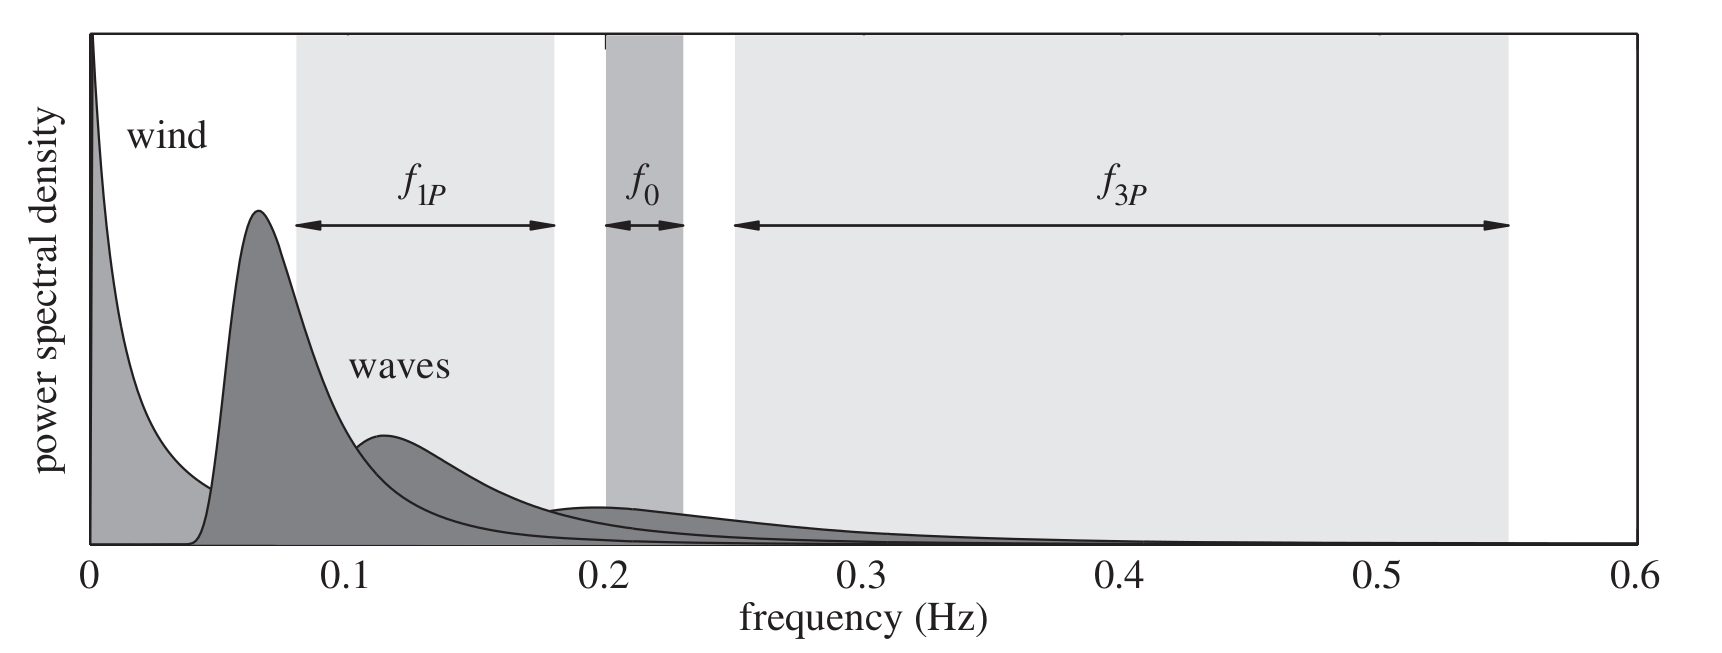
\includegraphics[width=0.75\textwidth]{./part1/figures/modal_analysis.png}
    \caption{Illustration of a soft-stiff design strategy, placing the structure's natural frequency $f_0$ away from the wind and wave power spectra, and the rotor excitation frequencies $f_{1P}$ and $f_{3P}$ (source: \citet{kallehave_2015_modal}).}
    \label{fig:modal_analysis}
\end{figure}

Modal analysis does not model transient loading phases and their corresponding non-linearities, which is crucial beyond early design. 
For a higher fidelity, simulations in the time domain using flexible multibody approaches are commonly used to describe the nonlinear dynamics \citep{holm_2009_multibody,alsolihat_2018_flexible_multibody}.
DIEGO implements such an approach by combining rigid multibody dynamics with a deflection model based on Lagrangian equations \citep{milano_thesis_2021}. 
Note that for floating wind turbines modeling, a preliminary step of rigid body dynamics is added to define the coordinate system of the floater. 
\citet{otter_2022_owt_modeling_review} reviews the state-of-the-art of numerical and experimental modelling techniques for multi-physics OWT systems.

\elias{Mention the Offshore Code Comparison Collaboration Continuation (OC4) project, for which a benchmark of OWT numerical models was realized around the academic DeepCwind concept proposed by the university of Maine}

%============================================================%
\subsection{Fatigue damage}
%============================================================%

Mechanical fatigue damage is an important phenomenon to consider when designing wind turbines. 
It refers to the progressive weakening of a material when subjected to cyclic or repeated loading, which may be significantly lower than the material's ultimate strength. 
Understanding the mechanisms behind mechanical fatigue damage is essential for designing durable and reliable structures. 
To quantify the fatigue damage on offshore wind turbine structures, standards \citep{dnv_fatigue_2016} recommend simulating the stresses in the time domain and identify a series of stress cycles. 
Then, the \textit{stress-number of cycles curve} of a specific material (S-N curve) gives the number of cycles before failure at a given constant stress amplitude. 
As the stress cycles identified on the results of the OWT simulation are not constant, an aggregation method called textit{Miner's rule} gathers the elementary damages over the stress time series studied. 


\paragraph{Stress cycles identification.}
%------------------------------------------------------------%
Offshore wind turbine simulators as DIEGO, deliver a time-dependent stress tensor. 
To ease the manipulation of this tensor, the equivalent Von Mises stress is computed, turning a multiaxial stress into an equivalent uniaxial stress. 
One can also consider a ``plane strain'' hypothesis on the Cauchy stress tensor $\underline{\underline{\sigma}}$, which is expressed as:
\begin{equation}
    \underline{\underline{\sigma}} = \begin{pmatrix}
                            \sigma_{11} & \sigma_{12} & 0\\
                            \sigma_{21} & \sigma_{22} & 0\\
                            0 & 0 & \sigma_{33}
                            \end{pmatrix}.
\end{equation}
This assumption simplifies the expression of the equivalent Von Mises stress: 
\begin{equation}
    \sigma _{\mathrm{VM}}=\sqrt{{\frac {1}{2}}\left[(\sigma _{11}-\sigma _{22})^{2}+(\sigma _{22}-\sigma _{33})^{2}+(\sigma _{33}-\sigma _{11})^{2}\right] + 3 \sigma _{12}^{2}}.
\end{equation}

Stress cycles can now be identified on the equivalent Von Mises stress time series. 
The usual method to identify fatigue stress cycles is caleld \textit{rainflow counting} \citep{dowling_1972}. 
Fatigue stress cycles are only defined by their amplitude (also called ``range'') and mean value, regardless of their chronology. 
Rainflow counting returns a list of stress ranges identified denoted by $s$ in the following. 


\paragraph{S-N curve.}
%------------------------------------------------------------%
The S-N curve is also called the ``W\"oler curve'' after the pioneer work of August W\"ohler, who demonstrated that fatigue damage was at the origin of railway accidents in the mid 19\textsuperscript{th} century \citep{schutz_1996_history_fatigue}. 
As a result of repeated fatigue experiments, this tool determines the number of similar stress cycles necessary to reach a fatigue ruin for a defined stress cycle amplitude. 
Its values depend on the material studied and on external conditions (i.e., in the offshore industry, the S-N curves distinguish the fatigue in the air vs. underwater). 

A well admitted simplification of the S-N curve is to consider it as log-linear on two segments:
\begin{equation}
\log(N_{\mathrm{c}}(s)) = \left\{
    \begin{array}{ll}
        \log(a_1) - m_1 \log(s), & \mbox{for}~ s \in [s_{\mathrm{min}}, s_{\mathrm{e}}] \\
        \log(a_2) - m_2 \log(s), & \mbox{for}~ s \in [s_{\mathrm{e}}, s_{\mathrm{max}}]
    \end{array}
\right.
\end{equation}
Where $N_{\mathrm{c}}$ is the predicted number of cycles to failure for stress range $s$, $m$ is the negative inverse slope of the S-N curve, 
$\log(a)$ is the intercept of log N-axis by the S-N curve, $s_{\mathrm{min}}$ is the minimal (resp. maximal) stress range identified by the rainflow counting, 
and $s_{\mathrm{e}}$ is the stress range axis of the intersection of the two log-lines formed by the S-N curve. 
The expression of this curve in two linear segments arise from the concept of endurance limit of a material, $s_{\mathrm{e}}$, under which the effect of fatigue on a material should be considerably smaller. 
According to \cite{dnv_fatigue_2016}, the S-N curve is altered for welded tubular joints by taking into account the tube's thickness:
\begin{equation}
N_{\mathrm{c}}(s) = \left\{
    \begin{array}{ll}
        a_{1} \left(s (\frac{t}{t_{\mathrm{ref}}})^h\right) ^{-m_1}, & \mbox{for}~ s \in [s_{\mathrm{min}}, s_{\mathrm{e}}]\\
        a_{2} \left(s (\frac{t}{t_{\mathrm{ref}}})^h\right)^{-m_2}, & \mbox{for}~ s \in [s_{\mathrm{e}}, s_{\mathrm{max}}]
    \end{array}
\right.
\end{equation}
With $t_{\mathrm{ref}}$ the reference thickness (for tubular welded joints $t_{\mathrm{ref}}$ = 25 mm); $t$ the plate thickness, and $h$ the thickness exponent.
The numerical values considered in the present work derive from the Section xx of \citet{dnv_fatigue_2016}, reproduced in the Table \ref*{tab:sn_table}.

\begin{table*}[h]
    \centering
    \caption{S-N curve numerical values of welded tubular joints in different environmental conditions (source: \cite{dnv_fatigue_2016})}
    \begin{tabular}{l|l|l|l|l|l}
     \hline
     \textit{Environment} & $m_1$ & $log(a_1)$ & $m_2$ & $log(a_2)$ & $h$\\
     \hline
     Air & $3.0$ & $12.48$ & $5.0$ & $16.13$ & $0.25$\\
     Seawater with cathodic protection & $3.0$ & $12.18$ & $5.0$ & $16.13$ & $0.25$\\ Seawater free corrosion & $3.0$ & $12.03$ & $3.0$ & $12.03$ & $0.25$\\ 
    \end{tabular}
    \label{tab:sn_table}
\end{table*}

\paragraph{Non-zero mean correction.}
%------------------------------------------------------------%
Most S-N curves are built over zero mean stress cycles, to consider different stress mean $s_m$, different empirical models were developed \citep{suresh_1998_fatigue_book}. 
The S-N curve becomes a three-dimensional envelope depending on the number of cycles $N_c$, the stress amplitude $s$, and the mean stress $s_m$. 
The ``Goodman line'' and the ``Gerber parabola'' are two models relating the stress amplitude $s$ to the mean stress $s_m$:  
\begin{align}
    \mathrm{Goodman} &:\quad \frac{s}{s_d} + \frac{s_m}{R_m} = 1\\
    \mathrm{Gerber} &:\quad \frac{s}{s_d} + \left(\frac{s_m}{R_m}\right)^2 = 1
\end{align}
Where the material's yield stress is denoted by $R_m$ and the fatigue limit by $s_d$. 
The Haigh diagram represented in the \fig{fig:haigh_diagram} is a slice of the three-dimensional envelope for fixed values of fatigue endurance (i.e., number of cycles).
By comparing the two models visually, the Goodman line is more conservative and is mostly used in the literature. 
Further discussion in the field of wind turbines were reviewed in the early 2000's with a focus on the fatigue endurance of glass fiber materials \citep{sutherland_2000_fatigueWT} 
In the present, the non-zero correction presented above are not considered as the values of mean stress were found to be negligible compared to the yield stress of the material studied. 

\begin{figure}
    \centering
    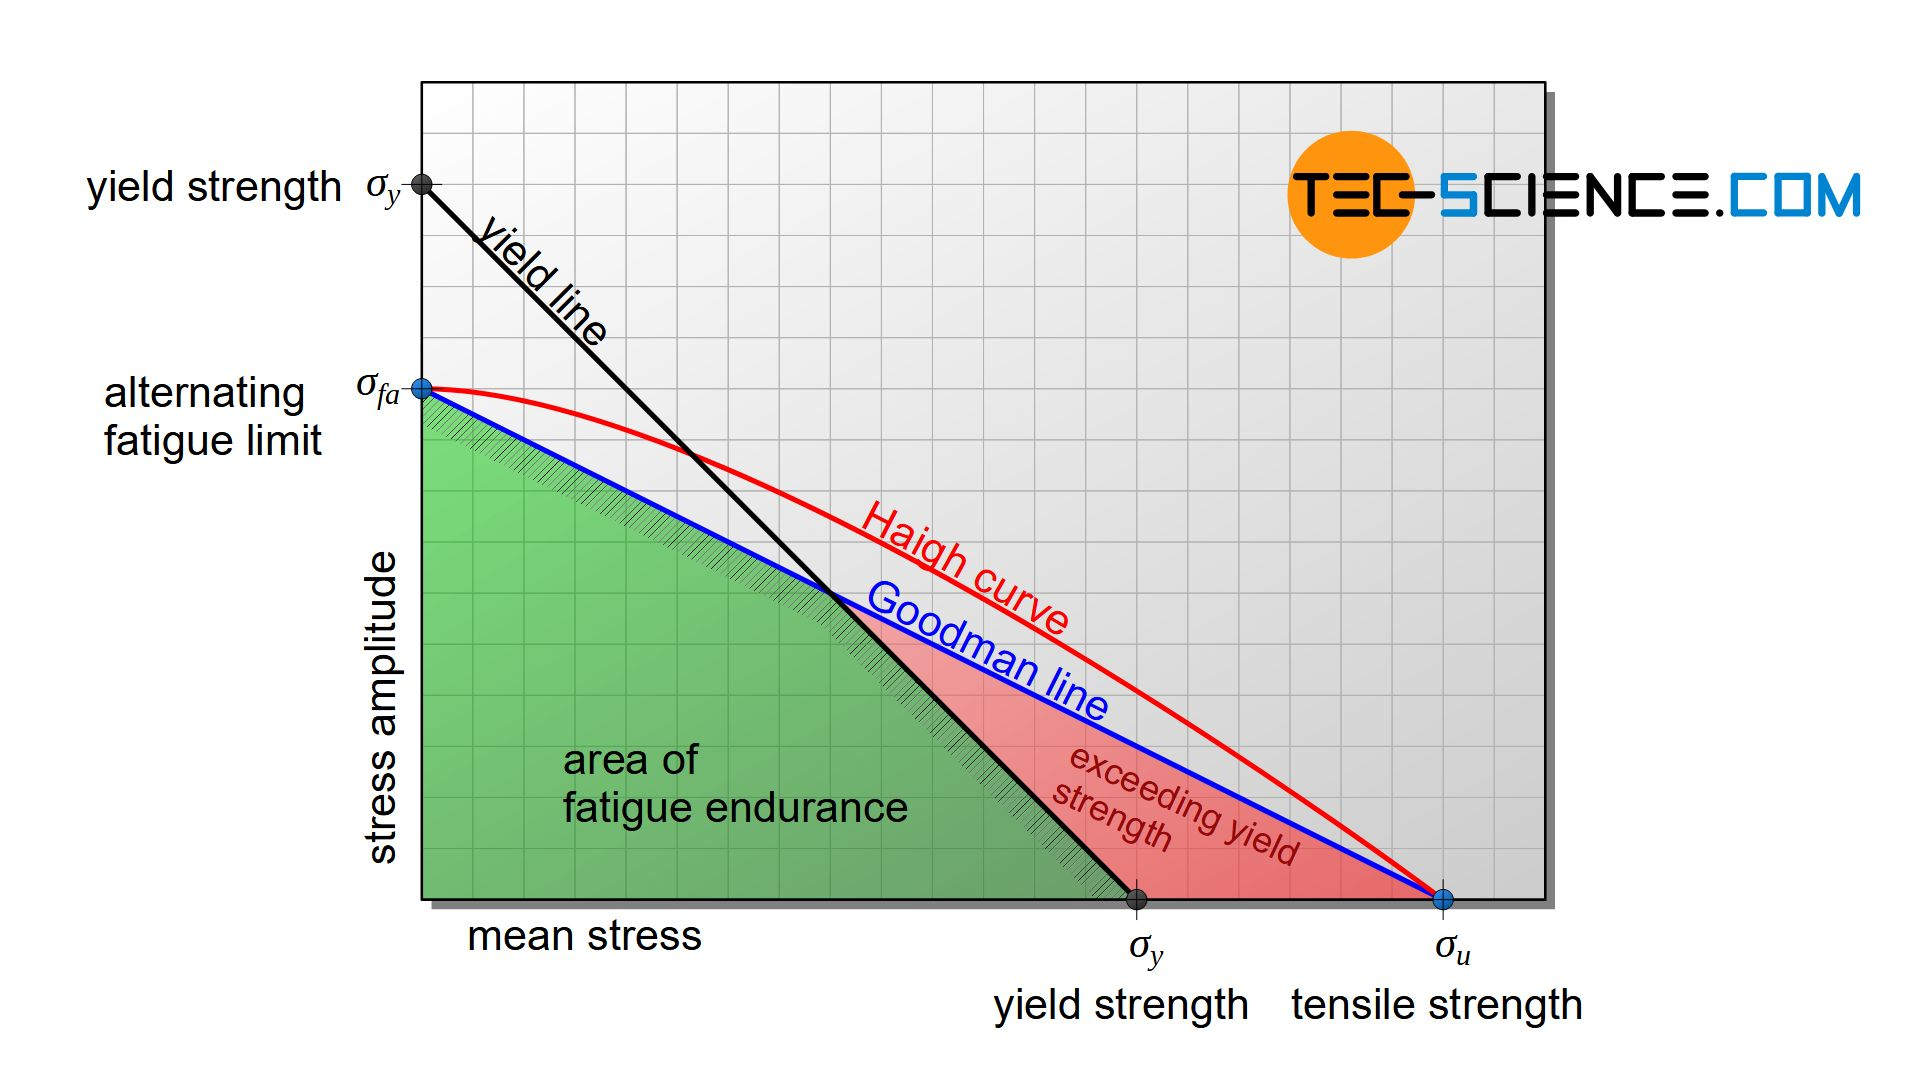
\includegraphics[width=0.7\textwidth]{./part1/figures/haigh-diagram.jpg}
    \caption{Illustration of the Haigh diagram representing the combination of stress mean and amplitude leading to the same fatigue endurance.\elias{Reproduce Haigh and Goodman in 3D}}
    \label{fig:haigh_diagram}
\end{figure}



\paragraph{Cumulative damage theory.}
%------------------------------------------------------------%
A popular approach to assess the damage cumulated on a stress time series is to consider the fatigue contribution of each stress cycle according to the S-N curve. 
Palmgren-Miner's rule defines the \textit{cumulative damage} $d_c$ by summing the fatigue contributions of each stress cycle $k$:
\begin{equation}
    d_c = \sum_{j=1}^{k} \frac{1}{N_{\mathrm{c}}\left(s^{(j)}\right)}.
    \label{eq:miner}
\end{equation}
In this theory, the material reaches fatigue ruin when the cumulative damage exceeds one.  
A common practice when using Palmgren-Miner's rule is to gather the stress cycles in a set of bins. 
This practice induces an integration error, which becomes significant as the number of bins is reduced. 
In the following, the cumulative damage is computed without binning, as defined in \eq{eq:miner}.


Spectral methods were also introduced to quantify fatigue damage in the late 80's. 
The main idea is to infer a PDF over the amplitudes of the stress cycles identified by rainflow counting, typically using a mixture of parametric distributions. 
From this PDF, one can derive the fatigue endurance and therefore a cumulated damage (further details in the review of \citet{dirlik_2021}). 
In the context of wind turbine fatigue assessment, spectral approaches showed to be unsuited in some cases, such as the fatigue of the blade's bending moments \citep{ragan_2007_dirlik_vs_miner}.  
Overall, fatigue estimation in the time-domain does not represent important computational effort compared to the simulation of the wind turbine's physics. 


%============================================================%
%============================================================%
\section{Design and operation practices} \label{sec:owt_design}
%============================================================%
%============================================================%

The design and operation of offshore wind turbines is at the intersection of various engineering, environmental and social considerations. 
Regardless of the different bottom-fixed or floating technologies, OWTs are dynamically excited structures evolving in a harch offshore environment.   
To operate such assets over up to 25 years of lifespan, multiple aspects should be assessed, from soil modeling, studies of environmental impact, grid integration, manufacturing quality, port logistics, to marine growth management, and maintenance
This section resumes the main types of OWT technologies, as well as the main design and operation practices.   

%============================================================%
\subsection{Types of technologies and preliminary design}
%============================================================%
Over the last two decades, multiple technologies of OWTs have been developped, which are generally gathered into two types: bottom-fixed or floating technologies. 
\fig{fig:FOWT_bottomfixed} and \ref{fig:FOWT_floating} respectively illustrates the diffrent types of bottom-fixed or floating technologies. 
At this stage, the bottom-fixed solutions present more maturity and the floating technologies are still transitionning from the phase of large demonstrators to large scale wind farms. 
The current developpement, in France, of offshore wind energy lead to the construction of the two first industrial projects, both managed by EDF Renewables \elias{(add the ADEME map of the offshore French project?)}. 
In Saint-Nazaire, 80 bottom-fixed wind turbines were built on monopile foundations, alltogether producing up to 480 MW \elias{add ref}. 
On the mediterannean coast, the first French industrial floating project was recently installed 20km offshore the coast of Marseille. 
This pilot project, called ``\textit{Provence grand large}'', is composed of three turbines operating on so called ``tension-leg platforms'', delivering 25 MW of nominal power installed.     

In order to lift water depth limitations associated with bottom fixed technologies (around 60 meters), floating pilot projects emerge accross the world. 
However, the wind energy industry still tests different floating technologies in terms of cost efficiency and durability (as listed in \citet{mackinnon_2022_FOWT_table}). 
An example of farm projects by type of technology is described hereafter: 
\begin{itemize}
    \item \textbf{Semi-submersible}: a pilot project of three 10MW turbines called ``\textit{les éoliennes du Golfe du Lion}'' in the south of France relies on a semi-submersible technology developped by the company Principle Power \citep{cermelli_2018_windfloat}.   
    \item \textbf{Tension-leg}: a pilot project of three 8MW turbines called ``\textit{Provence grand large}'' exploits tension-leg platforms co-developped between the IFPEN national laboratory and the company SBM \citep{caille_2017_TPL_IFPEN}. 
    \item \textbf{Barge}: a pilot project of three 10MW turbines called ``EOLMED'' uses the floater developped by the company Ideol \citep{guignier_2016_ideol}. 
    \item \textbf{Spar}: the Norvegian oil and gas company Equinor chose the spar technology \citep{driscoll_2016_hywind} to equip its floatting wind farm of 88MW, named ``Hywind Tampen''. 
\end{itemize}

\begin{figure}
    \begin{subfigure}[b]{0.48\textwidth}
        \centering
        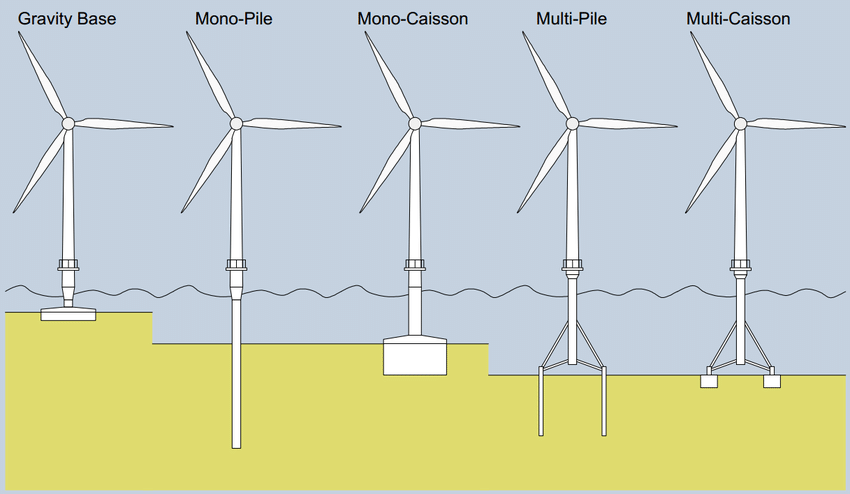
\includegraphics[width=\linewidth]{./part1/figures/bottom_fixed_techno.png}
        \caption{Bottom-fixed}
        \label{fig:FOWT_bottomfixed}
    \end{subfigure}
    \begin{subfigure}[b]{0.48\textwidth}
        \centering
        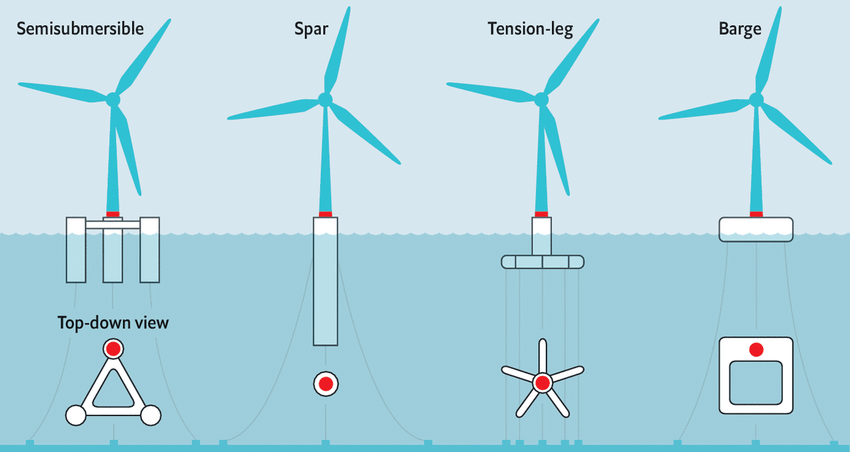
\includegraphics[width=\linewidth]{./part1/figures/Floating-wind-platform-categories.png}
        \caption{Floating}
        \label{fig:FOWT_floating}
    \end{subfigure}
    \caption{Main offshore wind turbine technologies (sources: \citet{ahmed_2015_bottomfixed_image,mei_2021_FOWT_illustration}).}
\end{figure}



The turbines installed offshore over bottom-fixed foundations or floating structures present the same properties and components. 
As described in \fig{fig:owt_diagram}, the structure of a wind turbine is composed of blades made in composite materials, while the tower, the transition peace and fundation (e.g., monopile) are made out of steel. 
\elias{Mention the steel type and the fact that catodic proection against the corrosition is usually used.}

Inside the nacelle, the gearbox adapts the rotation speed to suit the energy conversion system (i.e., generator). 
To improve the reliability of the components, manufacturers offer without gearboxes, called ``direct-drive''. 
This technology is relevant offshore, as the maintenance contraints are higher. 
However, the corresponding generators used in this situation operate at lower rotation speed. 
Adapting the generators significantly incease their weigth and requires the use of larger permanent magnets increasing their price.   

\begin{figure}
    \centering
    \elias{add diagram}
    
    \caption{Diagram of an offshore wind turbine's major components.}
    \label{fig:owt_diagram}
\end{figure}

The construction of an offshore wind farm requires several years of project planning, administrative procedures, consultation of the public opinion, and design. 
Internationals standards define the recommanded practice and requirements realted to the design and operation of OWTs. 
Among them, the IEC 61400 is subdivided in many parts, incluing the general one \citep{iec_2019} and other parts details specific topics.       
To validate the structural integrity of an wind turbine design, the standards recommand to simulate the behavior of the OWT (using the methods described in Section \ref{sec:owt_modeling}) for many environmental conditions, called ``design load cases'' (DLC). 
As the environmental conditions (i.e., the DLC) depend on the site studied, the standards provide generic DLCs depending on a rough classification of the environmental conditions. 
\elias{concepts of ULS and FLS + the standards provide a DLC for each of the main situations: parked / in prod etc.}
Advanced sampling methods reling envrionmental data measured on site will be introduced in Chapter 4. 
Beyond the main sollicitations resulting from environmental loading, various aspects should be considered around offshore wind turbines. 


%============================================================%
\subsection{Further design considerations}
%============================================================%
The present section focues on different topics to be adressed ahead or during the design and operation of offshore wind turbines.

\paragraph{Soil modeling.}
%------------------------------------------------------------%
The accurate geotechnical description of an offshore site plays an important role in the design and stability of bottom-fixed offshore wind turbines. 
The seabed soil properties are far from uniform in a wind farm, forcing the designer to adapt the fundations within a farm. 
Prior to the installation, geotechnical surveys and soil testing are conducted to assess parameters such as soil composition, density, strength, and seabed stability. 

To model the dynamic behavior of fondations, certification companies adapted their the methods from the oil \& gas industry to the offshore wind energy \citep{dnv_2018_soil}. 
For monopile fondations, the ``$p-y$'' method is often used to model soil-structure interactions. 
Assuming that these interactions are purely lateral, this method defines a set of non-linear lateral springs along the fondation's height.  
Together, the springs model the relation between the soil resistance ``$p$'' and the lateral displacement ``$y$''. 
Generally speaking, monopile foundations for OWT tend to be more rigid than for oil \& gas platforms, as the cyclic loading on wind turbines induces more fatigue (see the case-study presented in \citet{le_2014_geotech_casestudy}).  
However, various contributions in wind energy extended the use of $p-y$ curves to the case of multidirectional and irreversible displacements \citep{lovera_2019_thesis}. 
In summary, geotechnical considerations are essential for offshore wind turbine design, and the variability of soil properties within a wind farm necessitates a tailored approach to foundation design. 
Finally, the consideration of uncertainties in this field is still an open research topic \citep{reale_2021_OWT_soil_uncertainties}.

\elias{Describe the modeling method in DIEGO called the ``apparent fixity'', and the defined soil stiffness matrix. See Petrovska p.52.}


\paragraph{Marine growth.}
%------------------------------------------------------------%
The bio-colonization of offshore structures and submarine cables is a significant concern in the maintenance and operation of OWTs. 
Elements exposed to the colonisation of marine organisms, such as mussels, can cause several adverse effects. 
Firstly, the added weight increases the mass of the turbine and its foundation, potentially changing the dynamics of the systems and its strucutural integrity. \citep{ameryoun_2019_marine_growth,schoefs_2022_reliability_marine_growth}
Secondly, marine growth changes the roughtness at the surface of the submerged components, which can create fluctuating hydrodynamic loads and vibrations \citep{marty_2021_cable_marine_growth}. 
To limit its impact on the reliability of OWTs, this phenomenon is adressed with regular preventive cleaning measures as part of the maintenance planning. 


\paragraph{Global scour.}
%------------------------------------------------------------%
The large-scale erosion of seabed sediment around bottom-fixed offshore wind turbine foundations, also called ``global scour'', poses different problems. 
The stability of the foundation is first reduced, potentially leading to tilting. 
Moreover, the load distributions changes, causing uneven stresses and increased fatigue. 
Finally, submarine cable exposure increases the risk of damage and electrical faults. 
As global scour is a critical element of the long-term OWT reliability, various mitigation measures are reviewed in \citet{fazeres_2021_scour}, including scour protection, and scour-robust foundation design.


\paragraph{Port logistics.}
%------------------------------------------------------------%
In the installation and maintenance of such large scale systems, port logistics plays an important role considering the international supply chain involved. 
The coordination, transportation and assembly of massive wind turbine components, foundations, and supporting infrastructure requires meticulous planning and execution. 
In accordance, the costs of handling operations, and maintenance represent an important share of the \textit{levelized cost of energy} (LCOE) \citep{shields_2021_owt_lcoe}.  

In their review of OWT installation techniques, \citet{jiang_2021_owt_installation_review}, describe the foundations' and components' installation processes depending on the OWT technology. 
Because of their large scale, most structural assembly (e.g., blades, or floater) are done on dedicated port docks, making the port choice critical.  
The assembeled turbines are then transferred offshore with specialized vessels, such as installation jack-ups. 
Timing and synchronization are critical, as weather windows for handling operations can be limited.


\paragraph{Grid integration.}
%------------------------------------------------------------%
Unlike traditional centralized energy productions plants (i.e., nuclear and fossil), wind energy has considerable impact on the grid management. 
The intermittency of offshore wind generation, driven by variable wind conditions, disrupts the grid stability as the electricity supply fluctuates with the wind \citep{heier_2014_grid_integration}. 
Then, grid balancing becomes more complex as variable and distributed production sources are introduced.  
Wind turbine integration often require more flexibility from the grid, resulting in grid infrastructure upgrades (e.g., energy storage) and advanced grid management. 




\paragraph{Environmental impact and social acceptance.} 
%------------------------------------------------------------%
The fast development of offshore wind turbines in Europe raises questions regarding envrionmental and social impact. 
On the environmental part, the installation and operation disrupt marine ecosystems, as reviewed by \citet{galparsoro_2022_owt_ecological_impact}. 
Further studies should be realized to better understand the reliance of the ecosystems to this change. 
This industry also affects other marine activities (e.g., fishing or tourism), and costal landscapes, which needs to be discussed during the regional marine spacial planning. 
Finally, social acceptance of offshore wind projects varies across Europe, split between local disturbances and the regional economic activity generated.  


\paragraph{Manufacturing quality.}
%------------------------------------------------------------%
The manufacturing of structural wind turbine components is subject to several uncertainties that can affect the overall quality and performance of OWTs. 
For example, the manufacturing process of composite blades can lead to inconsistencies in the final product
Imperfections in the composite material, like air pockets or delamination, can weaken the blades and reduce their lifespan. 
Additionally, variations in manufacturing processes can result in differences in blade weight and balance, impacting turbine performance. 
Regarding steel components, OWTs are mostly assembeled by bolted and soldered joint. 
Inconsistent soldering, variations in material properties, and potential flaws in the joints can compromise the structural integrity of OWTs \citep{veers_2019_review}. 
These uncertainties in manufacturing quality can pose significant challenges in ensuring the reliability and longevity of the structures. 
Note that at the design phase, \textit{stress concetration factors} are defined by standards to take into account the local change in material properties created by soldering. 
Rigorous quality control, material testing, and manufacturing standards are essential to maintain the safety and efficiency of wind energy installations. 


\paragraph{Maintenance and end-of-life management.}
%------------------------------------------------------------%

To ensure the continued performance and availability of wind turbines, advanced maintenance planning is essential. 
Maintenance activities involve inspections, repairs, component replacements, and addressing issues as corrosion, or electrical faults. 
Preventive maintenance strategies reviewed by \citet{ren_2021_owt_maintenance}, minimizes the asset's unavailability and extends its lifespan. 

Once the wind farms reach their planned lifetime (typically around 20-25 years), the operator has the choice between decomissioning, ``repowering'', or ``revamping'' of the assets. 
Usually, revamping defines an intermediate renovation of a wind energy asset. 
In most cases, the underperforming major components are replaced while the structural components are kept. 
Alternateively, repowering is a strategy reusing the foundations of a wind farm to install brand new furbines. 
This approach is often an opportunity to increase the scale and performances of the old turbines. 

As the first generation of wind farms currently reach their end-of-life, an important problematic raises from recycling large amounts of blades made out of composite materials. 
Different processes for recycling composite material are reviewed in \citet{jensen_2018_blade_recycling}, including mechanical, pyrolysis and chemical techniques. 
However, recycling composites is a complex and energy-consuming operation, that needs to be further studied. 
The recent lifecycle study of floatting OWT in the mediterranean region by \citet {pulselli_2022_FOWT_lifecycle} showed that effective maintenance and 
proper decommissioning planning are essential for enssuring cost-effective yet durable lifecycle management.  




%============================================================%
%============================================================%
\section{Uncertain inputs} \label{sec:owt_uncertainties}
%============================================================%
%============================================================%

Following the general diagram of uncertainty quantification in \fig{fig:UQ_methodo}, this section focuses on the definition of the uncertain inputs and their corresponding probabilistic model (step B). 
In our case, the generic term of ``inputs'' refers to the inputs to the wind turbine numerical model illustrated in \fig{fig:owt_chained_model}, which will be considered as random afterwards. 

The random variables studied in this work are split into two groups, assumed independent, which are respectively called \textit{envrionmental variables} and \textit{system variables}. 
First, the environmental variables are a collection of variables caracterizing the long-term metocean conditions near a wind farm. 
As illustrated by the environmental dataset representing the conditions of a site located in the south of Brittany, \elias{Fig xx}, the underlying random vector presents a complex dependence structure. 
However, this source of variability is well known as the wind potential is well studied before and during a wind farm project.   

The second group of uncertain inputs is related to the wind turbine system. 
A wide range of uncertainties can be taken into account in such systems, such as material properties, manufacturing quality, soil conditions, control error, corrosion, marine growth, aerodynmic damping, etc.  
Among them, a restricted list of four variables are kept according to sensitivity analysis results from the literature and expert knowledge. 
The present section defines the two groups of random variables, including a focus on the definition of probabilistic S-N curves. 


%============================================================%
\subsection{Environmental inputs}
%============================================================%


During the planning and operation of a wind farm project, the metocean conditions are studied using different sources of information. 
At the early stage, datasets generated by fine mesoscale numerical simulation can be used to assess the wind potential. 
This was typically the case during the call for tenders\footnote{\url{https://eolbretsud.debatpublic.fr/}} issued by the French government regarding the construction of two floating offshore wind farm in the south coast of Brittany (of respectively 250 and 500 MW of nominal power). 
Open-access environmental data of the sea-states in this reagion were available, as a result of mesoscale simulations \citep{raoult_2018_anemoc3} realized by EDF R\&D.    
In a second time, to get a local assessment of the conditions, a meteorological mast with wind speed cup anemometers at different heights and wave boy are generally installed in the vincity of the future farm. 
As a cheaper alternative to met mast, new measurement technologies such as floating LIDARs (for light detection and ranging) are significantly cheaper \citep{gottschall_2017_floating_LIDAR}. 
The adequation of the local measures with the data obtained by mesoscale simulations  to imporove wind assessment is reviewed in \citet{sempreviva_2008_wind_assessment_review}.  
Finally, after the installation of the turbines, the acquisition system (usually called SCADA, for ``Supervisory Control And Data Acquisition'') measure wind conditions with a sampling period of ten minutes. 

In the present work, two wind farms projects are partially studied: the Teesside wind farm, operating in the North Sea, and the south Brittany floatting project, at the stage of tenders call. 
Table \ref{tab:envi_variables} summarizes the variables considered as random hereafter. 
The inference of such data will be discussed in the upcoming Section \ref{sec:32_inference}. 
Note that the environmental data resulting from the SCADA system of the Teesside wind farm is confidential, and will be represented as anonymized data in the following. 

\begin{table}[h!]
    \centering
    \begin{tabular}{ l l l}
        \hline
        {\it Name} & {\it Notation} & {\it Description}\\
        \hline
        Mean wind speed & $U$ & 10-min. average horizontal at 10m\\
        Turbulence & $\sigma_s $ & 10-min.  standard deviation \\
        Wind direction & $\theta_{wind} $ & Wind directions\\
        Significant wave height & $H_s $  & Significant wave height per hour\\
        Peak wave period & $T_p $ & Peak 1-hour spectral wave period \\
        Wave direction & $\theta_{wave} $ & Wave directions\\
        %Mean shear & $\alpha$ & Normal & 10-min mean shear exponent \\
        %Air density & $\delta$ & - & -\\
        \hline
    \end{tabular}
    \caption{Marginal distributions of the environmental random variables}
    \label{tab:envi_variables}
\end{table}

%============================================================%
\subsection{System inputs}
%============================================================%
As mentionned earlier, multiple parameters in a wind turbine system can be considered as uncertain. 
Our study focuses on the effects of uncertainties on the fatigue damage over the structure. 
Therefore, the litterature review of the sensitivity analysis on offshore wind turbine fatigue helped us narrow down a few system variables. 
Petrovska explored the sensitivity analysis of many variables on the fatigue of a wind turbine in Teesside. 
Even if the use of the Morris method is questionable, as discussed in \citet{petrovska_2022}, the results allowed to screen some variables. 
For example, the uncertainties related to the corrosion, the wind shear exponent, or the nacelle mass showed a limited impact on the fatigue.     
By crossing the conclusions of various research, including \elias{add list}, with the expert knowledge among partners from the HIPERWIND european project, the system variables considered uncertain in the following are summarized in Table \ref{tab:sys_variables}.
Each of them is assumed independent, with a marginal probabilistic model arising from the literature. 

\elias{explain the resistance}

\begin{table}[h!]
    \centering
    \begin{tabular}{ l l l l}
        \hline
        {\it Name} & {\it Notation} & {\it Marginal model} & {\it Description}\\
        \hline
        Soil coefficient & $S$ & Normal ($\mu=1., \sigma=0.3$) & Applied to the soil stiffness matrix\\
        Yaw misalignment & $\theta_{\mathrm{m}}$ & Normal ($\mu=0., \sigma=0.3$) & [deg.] \\
        SN curve coefficient & $a$ & Log-normal ($\mu=1, \sigma=0.3$) & See \cite{guede_2007}\\
        Resistance & $D_{\mathrm{cr}}$ & Log-normal ($\mu=1, \sigma=0.3$) & See \cite{drexler_musculus_2021}\\\hline
    \end{tabular}
    \caption{Marginal distributions of the system random variables}
    \label{tab:sys_variables}
\end{table}



\subsection{Probabilistic fatigue assessment}
%------------------------------------------------------------%
The definition of a fatigue endurance model prime impact on fatigue damage assessment. 
However, the S-N curves usually describing the endurance of a material are built from repeated laboratory experiments, source of variability. 
Even if the need for random S-N curves has long been expressed in the field of fatigue experiments \citep{lieurade_1982_essais_fatigue}, their probabilistic description was better formalized in \citep{guede_2007,sudret_2013_fatigue}. 

The models proposed in \citet{guede_2007} are based on the experimental procedure used to build the S-N curves. 
For a given steel specimen, a cyclic loading (e.g., pure traction) is repeated with fixed amplitude until fatigue ruin. 
Because of variations in the material's microstructure, the fatigue endurance for the same cyclic solicitation is random. 
This variation is commonly assumed to follow a log-normal distribution in the literature. 
A probabilistic model of the S-N curve naturally comes: 
\begin{subequations}
    \begin{align}
        \log(N_c(s, \omega)) &= \log(a) - m \log(s) + \log(\varepsilon(\omega))\\
        \Rightarrow N_c(s, \omega) &= a \, s^{-m} \, \varepsilon(\omega),
    \end{align}
\end{subequations}

where $\log(\varepsilon(\omega)) \sim \mathcal{N}(0, 0.2)$. 

This uncertainty can be injected in the Miner-Palmgren rule defined in \eq{eq:miner}: 
\begin{equation}
    d_c(\omega) = \sum_{j=1}^k \frac{1}{N_c(s^{(j)}, \omega)}
            = \sum_{j=1}^k \frac{1}{a \, \left(s^{(j)}\right)^{-m} \, \varepsilon(\omega)}
            = \frac{1}{\varepsilon(\omega)} \sum_{j=1}^k \frac{1}{a \, \left(s^{(j)}\right)^{-m}}
\end{equation}
Note that the consideration of this uncertainty can be assessed as a pure post-processing of fatigue damage results computed with a deterministic S-N curve. 
In the wind energy standards, design S-N curve are actually a conservative envelope of the measured fatigue endurance. 
For example, the Annex F.7 in \citet{dnv_fatigue_2016} gives recommendations to define a design S-N curve from fatigue measures. 
Assuming that the fatigue endurance follows a Gaussian distribution (on logarithmic scale), the design S-N curve is the curve as two standard deviations below the mean curve. 
\fig{fig:probabilistic_SN} illustrates the design curve defined by DNV for tubular joints (in Section 2.4.6) and the reconstructed probabilistic model assuming a standard deviation equal to \elias{check the value use}. 

\begin{figure}
    \centering
    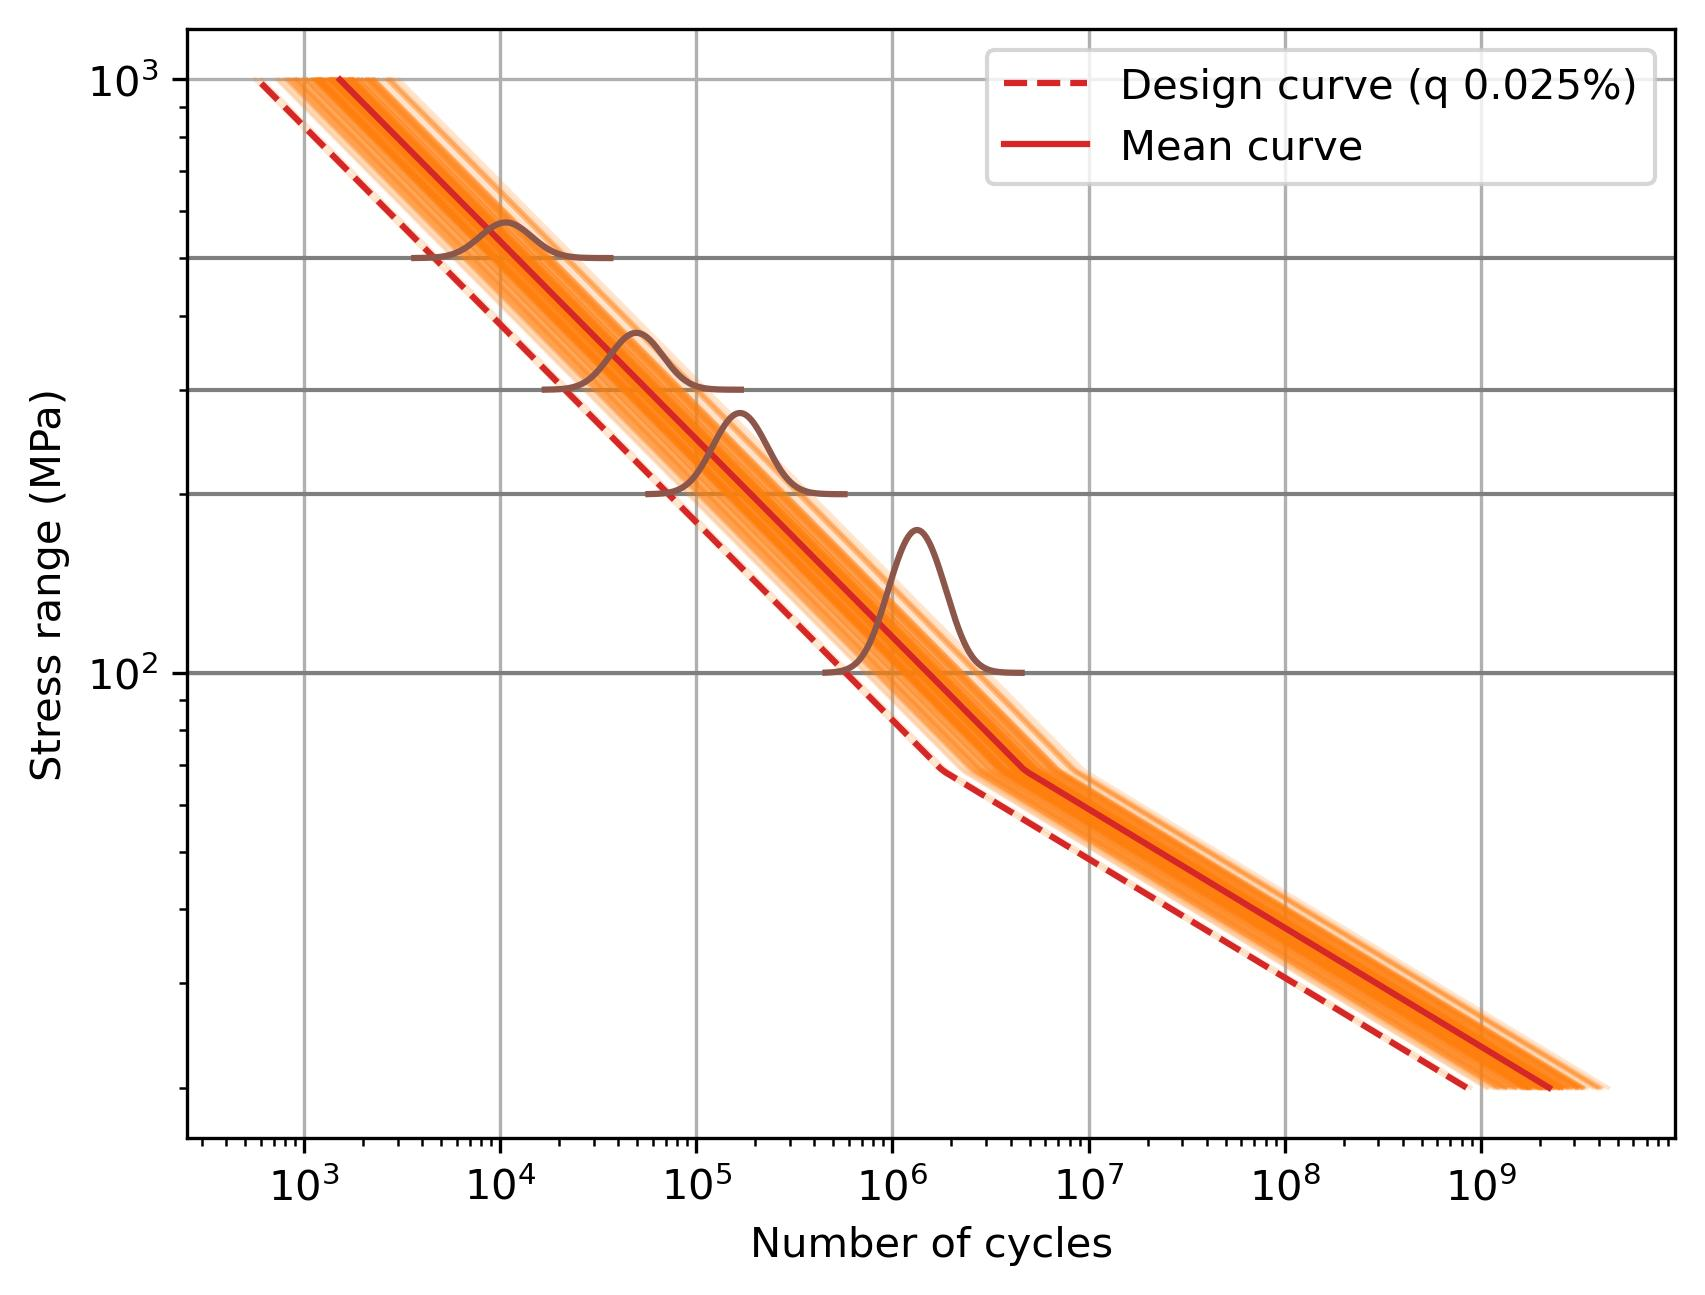
\includegraphics[width=0.6\textwidth]{./part1/figures/probabilistic_fatigue.jpg}
    \caption{Illustration of a probabilistic S-N curve according to the model defined in \citet{guede_2007}.}
    \label{fig:probabilistic_SN}
\end{figure}


%============================================================%
%============================================================%
\section{Conclusion}
%============================================================%
%============================================================%



